% options:
% thesis=B bachelor's thesis
% thesis=M master's thesis
% czech thesis in Czech language
% english thesis in English language
% hidelinks remove colour boxes around hyperlinks

\documentclass[thesis=M,czech]{FITthesis}[2012/06/26]

\usepackage[utf8]{inputenc} % LaTeX source encoded as UTF-8

\usepackage{graphicx} %graphics files inclusion
% \usepackage{amsmath} %advanced maths
% \usepackage{amssymb} %additional math symbols

\usepackage{dirtree} %directory tree visualisation

% % list of acronyms
% \usepackage[acronym,nonumberlist,toc,numberedsection=autolabel]{glossaries}
% \iflanguage{czech}{\renewcommand*{\acronymname}{Seznam pou{\v z}it{\' y}ch zkratek}}{}
% \makeglossaries

\newcommand{\tg}{\mathop{\mathrm{tg}}} %cesky tangens
\newcommand{\cotg}{\mathop{\mathrm{cotg}}} %cesky cotangens

% % % % % % % % % % % % % % % % % % % % % % % % % % % % % % 
% ODTUD DAL VSE ZMENTE
% % % % % % % % % % % % % % % % % % % % % % % % % % % % % % 

\department{Katedra softwarového inženýrství}
\title{Mobilní platforma pro podporu vykonávání aktivit řízená aktuálním kontextem}
\authorGN{Bohuslav} %(křestní) jméno (jména) autora
\authorFN{Mach} %příjmení autora
\authorWithDegrees{Bc. Bohuslav Mach} %jméno autora včetně současných akademických titulů
\supervisor{Ing. Zdeněk Míkovec, Ph.D.}
\acknowledgements{
Rád bych poděkoval především vedoucímu práce panu Ing. Zdeňku Míkovcovi, Ph.D. za jeho rady a pomoc při tvorbě tohoto textu a panu Ing. Janu Balatovi za jeho vstřícnost a umožnění uživatelských rozhovorů. Dále bych rád poděkoval svým blízkým a přátelům za velkou podporu, kterou mi projevovali po celou dobu mého studia.
}
\abstractCS{
Tato práce se zabývá problematikou tvorby mobilní platformy pro efektivní spouštění aplikací v závislosti na 
pravidelným aktivitách. Cílem je vytvořit aplikaci pro mobilní zařízení, která přináší inovativní vylepšení stávajících řešení, se zaměřením na limitované uživatele.

V první části text detailněji popisuje tento problém, vymezuje cíle práce, podává přehled o stávajících řešeních a vývojových platformách. Dále popisuje provedený návrh řešení, požadavky na funkcionalitu aplikace a na některé implementační části. Následující část čtenáři přiblíží vlastní implementaci aplikace a její testování v průběhu vývoje. V závěrečné části je pak výsledná práce zhodnocena a nastíněna práce budoucí.
}
\abstractEN{
Sem doplňte ekvivalent abstraktu Vaší práce v~angličtině.
}
\placeForDeclarationOfAuthenticity{V~Praze}
\declarationOfAuthenticityOption{1} %volba Prohlášení
\keywordsCS{Launcher, Accessibility, Kontext, Mobilita}
\keywordsEN{Nahraďte seznamem klíčových slov v angličtině oddělených čárkou.}

\begin{document}

% \newacronym{CVUT}{{\v C}VUT}{{\v C}esk{\' e} vysok{\' e} u{\v c}en{\' i} technick{\' e} v Praze}
% \newacronym{FIT}{FIT}{Fakulta informa{\v c}n{\' i}ch technologi{\' i}}

\begin{introduction}
Mobilní zařízení se v posledních letech stala nedílnou součástí našich životů a není nadsázkou, řekneme-li, že si svůj běžný den bez těchto moderních vymožeností nedokážeme představit. Obyčejné aktivity, jako zasílání textových zpráv nebo uskutečnování a přijímání hovorů, si už ani neuvědomujeme. Vyřizování emailů, hledání spojení nebo rezervaci oblíbené restaurace můžeme pohodlně realizovat prostřednictvím mobilních aplikací, rychle a jednoduše. Díky tomu mnoho uživatelů již nepotřebuje osobní počítač a všechny potřebné úkony vyřídí přes svůj mobilní telefon nebo tablet.

Počet aplikací se každým dnem zvyšuje a my objevujeme stále více takových, které nám usnadní každodenní úkony. Jejich instalace je díky specializovaným internetovým obchodům velmi jednoduchá a proto nikdo z nás nepřemýšlí nad tím, kolik jich vlastně v telefonu má. S rostoucím počtem nainstalovaných aplikací se stává hlavní menu čím dál tím víc nepřehledné a hledání zdlouhavější a obtížnější. Určitou formou řešení může být sdružení podobných/oblíbených aplikací do složek, čímž časovou ztrátu při hledání zmenšíme. Méně zkušení uživatelé však nemusí být s těmito možnostmi obeznámeni a jakékoliv složitější operace je mohou odradit.

Je tu však další skupina, které tento způsob nemusí tak úplně vyhovovat. Představme si uživatele, který se z nějakého důvodu nachází v časové tísni. Potřebuje otevřít aplikaci ihned a nemůže mobilnímu zařízení věnovat příliš mnoho času. Do takových situací se pravidelně dostávají například řidiči a ačkoliv se to na první pohled nezdá, tak do této skupiny patří určitým způsobem i zrakově postižení. Při práci s mobilním zařízením nejsou běžné operace pro vidícího člověka žádný problém. Proto například vybrat položku v menu nezabere díky vizuálnímu vjemu zdaleka tolik času, jako kdybychom všechny položky museli projít jednu po druhé.

Tímto způsobem však musí se seznamy pracovat každý zrakově postižený uživatel. Díky tomu se může dostat do časové tísně daleko snáze, protože operace, která vidícím uživatelům zabere pět minut, trvá této skupině zpravidla několikrát déle. Proč bychom tedy nemohli pravidelně vyhledávané položky řadit na začátek seznamu a nejlépe ty, které by mohl uživatel potřebovat právě v tuto chvíli (v aktuálním kontextu)? Převedeme-li tento požadavek na problém vyhledávání a spouštění aplikací, tak by uživateli v ideálním případě stačilo projet prvních několik položek, ve kterých by našel požadovanou volbu. Časová úspora by tak mohla být velmi znatelná. Samozřejmostí je, že by tento způsob byl efektivní i pro ostatní uživatele, kteří by tak měli vhodné aplikace ihned na očích a nemuseli by zdlouhavě projíždět menu nebo sdružovat aplikace do složek.

Jak vyplývá z předchozích odstavců, tak aplikace, která by nahradila klasickou domácí obrazovku její chytřejší verzí, by usnadnila práci a ušetřila čas širokému spektru uživatelů, především pak těm, kteří se potýkají s některou formou limitace. V následujícím textu se tedy budeme zabývat návrhem a implementací takového systému, který by měl být pro uživatele maximálně komfortní a přívětivý.

\section{Popis problému, specifikace cíle}

V této kapitole se pokusíme nastínit rozsah aplikace a dané problematiky. Nejdříve zmíníme samotné oficiální zadání této práce, poté si přiblížíme pojmy, které se budou nejčastěji objevovat v souvislosti s vývojem aplikace. Jako poslední podkapitola nás čeká vymezení cílů práce, které nám budou sloužit pro představu, jaké úkoly nás budou při implementaci čekat.

\subsection{Popis problému}

Cílem práce je vytvořit software pro uživatele \uv{chytrých} telefonů, který jim umožní efektivnější spouštění aplikací díky sledování jejich pravidelného režimu. Během vývoje bychom měli analyzovat potřeby a požadavky specifických cílových skupin s omezenou možností interakce (zrakově a pohybově postižení, řidiči atp.). Dále bychom se měli seznámit s vývojovými platformami, které mohou být reálně využity vzhledem k cílovým skupinám a provést analýzu kontextu v závislosti například na poloze, časových údajích, událostech v kalendáři, spouštěných aplikacích, probíhajících činnostech aj.

Na základě těchto údajů se pokusíme navrhnout platformu využívající aktuální kontext pro generování nabídky a spouštění uživatelských aktivit v podobě dostupných aplikací na koncovém zařízení. Zaměříme se na přívětivost a srozumitelnost grafického rozhraní a chování aplikace pro cílového uživatele.

\subsection{Definice pojmů}

Vytvoření definice pojmů, který bude shrnovat nejčastější pojmy spojené s vývojem aplikace, je velmi důležité z důvodu lepší a snadnější orientace čtenáře v celém textu. Jedná se vlastně o formu výkladového slovníku, jenž pomůže především těm, kteří jsou méně znalí dané problematiky. Pro tuto skupinu by se totiž výsledná práce mohla stát matoucí a těžko pochopitelnou.

\begin{description}
\item[Uživatel] je entita, která nějakým způsobem interaguje s naší aplikací a využívá ji.
\item[Launcher] je domácí (hlavní) obrazovka, kterou uživatel vidí ihned po plnohodnotném spuštění operačního systému.\cite{launcher}
\item[Aplikace] je programové vybavení mobilního zařízení. Jedná se například o emailového klienta, internetový prohlížeč nebo přehrávač hudby.
\item[Senzor] je zdroj informací o stavu mobilního zařízení nebo jeho okolí. Například se může jednat o teploměr, GPS nebo Wi-Fi modul.
\item[Data] jsou informace získané ze senzorů. Například okolní teplota, poloha mobilního zařízení nebo seznam dostupných Wi-Fi sítí.
\item[Platforma] určuje použitý operační systém, knihovny, ale i použité programovací jazyky či kompletní framework (vývojová a běhová platforma).\cite{platform}
\item[Accessibility] definuje míru dostupnosti určitého produktu definované skupině uživatelů. V našem případě se s tímto pojmem setkáváme především ve spojení se zrakově postiženými uživateli.
\item[Aktivity] jsou uživatelská činnosti, které budeme monitorovat a ve kterých se budeme snažit hledat pravidelnosti a šablony.
\item[Kontext] vyjadřuje aktuální stav, ve kterém se nachází mobilní zařízení a prostředí okolo něj.
\end{description}

Takto zadefinované pojmy nám pomohou lépe se orientovat v probírané problematice a předejít případným záměnám a omylům.

\subsection{Vymezení cílů práce}
Jednotlivé cíle práce jsme v širším pohledu zmínili již v předchozích kapitolách. Během návrhu a vývoje aplikace chceme klást důraz na reflektování potřeb a zachycení pravidelného režimu specifických skupin uživatelů (zrakově postižení). Na jejich základě vybrat nejvhodnější budoucí platformu, která by jim i vývojářům poskytovala co nejkomfortnější služby, a detailně analyzovat vnitřek budoucího systému s důrazem na nízkou provázanost, vysokou flexibilitu a jednoduchou rozšiřitelnost vzhledem k předpokládané další práci.

Rozepsat v analyze funkcni nefunkcni pozadavky? nebo zde sepsat oblasti, ktere je potreba vyresit? (Jak se budou aplikace radit, jak se budou shromazdovat informace atp.)

\end{introduction}

\chapter{Analýza a návrh}
Správná a dostatečně detailní analýza projektu bude stěžejní součástí tohoto textu a výsledného produktu. Nejprve se budeme věnovat uživatelskému výzkumu, díky kterému budeme schopni modelovat pravidelný cyklus naší cílové skupiny. Popíšeme si jak by měla vypadat architektura systému a provedeme rešerši mobilních platforem...?

\section{Uživatelský výzkum}
Stěžejní částí naší práce je uživatelský výzkum uskutečněný, mimo jiné, ve spolupráci s ČVUT FEL, katedrou počítačové grafiky a interakce. Informace z provedených rozhovorů nám pomohou nahlédnout do světa uživatelů, pro které naši aplikaci vyvíjíme, a pochopit jejich potřeby a požadavky. Výstupním produktem pak bude sestavení pravidelného týdenního cyklu, který nám pomůže odhalit s jakým druhem problému se budeme reálně potýkat.

\subsection{Interview}
Seznam následujících několik otázek, které by nám měly pomoci získat od uživatelů potřebné informace pro další vývoj, sloužil jako volnější osnova v závislosti na směru, kterým se rozhovor ubíral. Výsledný počet položek byl během několika iterací (před započetím rozhovorů) redukován a jejich znění mírně upravováno vzhledem k tomu, že na jednotlivé rozhovory bylo vymezeno časové rozhraní cca 10-15 minut.

Dotazy nebyly omezeny pouze na mobilní zařízení, ale brali jsme v potaz i osobní počítač, jelikož mnoho dotazovaných používá různé počítačové programy, jejichž funkcionalitu ale dokáží plnohodnotně zastat i aplikace pro mobilní telefony/tablety.

\begin{enumerate}
\item Jakého druhu je Vaše limitace?
\item Jak dlouho se s touto limitací potýkáte a kdy k ní došlo? (od narození, v dětství, později)
\item Jaký typ mobilního zařízení využíváte?
\begin{enumerate}
\item Uvažoval/a jste o přechodu na dotykové mobilní zařízení?
\end{enumerate}
\item Jaký je Váš pravidelný režim? (denní, týdenní, dvoutýdenní atp.)
\item Jaké jsou Vaše typické (opakované) činnosti? (cesty, venčení, pořady, práce atp.)
\item Jaké aplikace nejvíce využíváte a kdy? (volání, SMS, kalendář, internet, spoje atp.)
\item Jaké plusy/mínusy jste při jejich používání zaznamenal/a?
\item Které z nich se Vám nejlépe používají a proč?
\item Na jaké problémy při jejich používání narážíte?
\item Existují aplikace, které jste z nějakého (jakého) důvodu přestal/a používat?
\end{enumerate}

\subsection{Vzorové scénáře}
Na základě uživatelského výzkumu si v následujících podkapitolách budeme schopni popsat pravidelné režimy našich cílových skupin. Jedná se o uměle vytvořené ideální scénáře (vytvoření prototypů), které jsou složené ze všech participantů dané skupiny s přihlédnutím k logickému uspořádání aktivit. Z takto popsaných scénářů a jejich aktivit odehrávajících se v rámci dne/týdne můžeme vypozorovat, jak bude vypadat reálný problém, který se snažíme pokrýt, v praxi a jak se bude naše aplikace v průběhu času schopna učit.

\subsubsection*{Rozčlenění aktivit}
Abychom mohli lépe odhadnout horizont učení, stanovili jsme si několik kritérií pro určitou formu kategorizace jednotlivých aktivit. Jmenovitě to jsou četnost, pravidelnost a variabilita. Na základě takto zvolených údajů můžeme přibližně stanovit, jak dlouho bude aplikaci trvat vysledování jednotlivých pravidelností v rámci našeho scénáře.

\subsubsection*{Četnost a pravidelnost}
Zcela záměrně uvádíme tato dvě kritéria ve společné kapitole, protože spolu velice úzce souvisí, jak si následně vysvětlíme. Zjednodušeně se dá na úvod říci, že čím četnější a pravidelnější aktivita, tím lépe a rychleji se ji bude aplikace schopna naučit.

Sledováním četnosti výskytu dané aktivity ve scénáři získáme přehled o cyklech, ve kterých se jednotlivé činnosti objevují, a také o tom, jaký má uživatel režim. Ty, které se vyskytují denně se bude aplikace schopna učit podstatně rychleji, než například ty, které se vyskytují jednou týdně nebo dokonce měsíčně. Díky stanovení pravidelnosti budeme mít přehled o tom, jak obtížné bude pro aplikaci najít tyto pravidelné cykly v záplavě sledovaných dat. Ideálním případem je pro nás absolutně pravidelný výskyt bez mezer (časových úseků vybočujících z pravidelného řádu).

V takovém případě bude aplikace schopna rozpoznat denní aktivitu během 2-3 dní, podobně týdenní během 2-3 týdnů. Můžeme tento odhad zobecnit tím, že si určíme časovou jednotku (den, týden, měsíc atp.). Následně pak bude platit, že se danou aktivitu aplikace naučí během dvojnásobku až trojnásobku této časové jednotky (příslušné její četnosti). Samozřejmostí je, že pokud například uživatel spouští aplikaci s pravidelností

\begin{itemize}
\item první den ano,
\item druhý a třetí den ne,
\item čtvrtý a pátý den opět ano,
\end{itemize}

tak se v takovém případě prodlouží doba učení na 4-5 dní, ačkoliv se jedná o aktivitu s denní četností. Navíc se může jednat buď o aktivitu, která má být spouštěna pouze ve všední dny, nikoliv o víkendu, nebo ji jen uživatel \uv{zapomněl} druhý a třetí den spustit.

Četnost výskytu budeme hodnotit slovně podle příslušného časového úseku, např. denní, týdenní, měsíční atp. Pravidelnost výskytu aktivity budeme hodnotit číselně na stupnici od jedné do pěti, přičemž jedna znamená pravidelná a pět znamená nepravidelná.

\subsubsection*{Variabilita}
Výskyt aktivity může a nemusí být striktně vázán na časové období (poslech zpravodajské relace versus čtení knihy). Zde proto přichází ke slovu variabilita, která bude popisovat tento fakt striktně z pohledu časového ukotvení. Opět platí, že aplikaci se budou lépe rozpoznávat aktivity s menší variabilitou v čase, jako je například zmíněné sledování/poslech hlavní zpravodajské relace nebo pravidelného pořadu (pevný čas).

Variabilitu výskytu budeme popisovat na stupnici od jedné do pěti (podobně jako u pravidelnosti), přičemž jedna udává pevný čas a pět naproti tomu velké časové rozmezí.

\subsubsection*{Nevidomí}
V prvním scénáři se pokusíme popsat možný pravidelný rytmus nevidomého člověka tak, jak jsme ho zaznamenali během našich rozhovorů.

\paragraph{Všední den}
\begin{itemize}
    \item \textbf{6:00 - 7:00} - vstávání
\begin{itemize}
        \item četnost: denní | pravidelnost: 1 | variabilita: 2
\end{itemize}
    \item vypravení dítěte do školy, poslech rádia, kontrola emailů, snídaně, venčení psa
\begin{itemize}
        \item nabídnutí aplikace pro poslech rádia, emailového klienta, aplikace s počasím
        \item četnost: denní | pravidelnost: 1 | variabilita: 1-2
\end{itemize}
    \item \textbf{8:30} - poslech pravidelného pořadu “Jak to vidí” na ČRo 2
\begin{itemize}
        \item nabídnutí aplikace pro poslech rádia (vstupní parametr - frekvence ČRo 2)
        \item četnost: denní | pravidelnost: 2 | variabilita: 1
\end{itemize}
    \item práce/aktivita
\begin{itemize}
        \item nabídnutí aplikace kalendář (denní přehled klientů)
        \item po skončení aktivity s klientem nabídnout aplikaci pro vystavení účtu
        \item preferování aplikací využívaných při práci
        \item četnost: denní | pravidelnost: 1 | variabilita: 2
\end{itemize}
    \item oběd, venčení psa
\begin{itemize}
        \item četnost: denní | pravidelnost: 1 | variabilita: 3
\end{itemize}
    \item práce/aktivita
\begin{itemize}
        \item preferování aplikací využívaných při práci
        \item četnost: denní | pravidelnost: 1 | variabilita: 2
\end{itemize}
    \item \textbf{19:00} - poslech zpráv na ČT24
\begin{itemize}
        \item nabídnutí aplikace pro sledování ČT24 / internetového prohlížeče (vstupní parametr - URL živého vysílání)
        \item četnost: denní | pravidelnost: 1-2 | variabilita: 1
\end{itemize}
    \item večeře, venčení psa
\begin{itemize}
        \item četnost: denní | pravidelnost: 1 | variabilita: 3
\end{itemize}
    \item četba, poslech televize/rádia, internet
\begin{itemize}
        \item nabídnutí aplikace pro poslech rádia / sledování televize, čtečky knih / aplikace pro přehrávání namluvených knih, internetového prohlížeče
        \item preference aplikací využívaných při relaxaci
        \item četnost: denní | pravidelnost: 1-2 | variabilita: 3
\end{itemize}
\end{itemize}

\paragraph{Úterý a čtvrtek}
\begin{itemize}
    \item \textbf{18:00} - vaření večeře
\begin{itemize}
        \item nabídnutí aplikace s recepty (ve spojení s chytrou lednicí by mohl být vstupním parametrem seznam potravin)

        \item četnost: týdenní | pravidelnost: 1-2 | variabilita: 2
\end{itemize}
\end{itemize}

\paragraph{Pátek}
\begin{itemize}
    \item \textbf{14:00} - španělština po Skype
\begin{itemize}
        \item nabídnutí aplikace Skype (alternativně se vstupním parametrem pro přímé volání kontaktu)

        \item četnost: týdenní | pravidelnost: 2-3 | variabilita: 1-2
\end{itemize}
\end{itemize}

\paragraph{Sobota}
\begin{itemize}
    \item \textbf{10:00 - 11:00} - odjezd na plavání a 12:00 - 13:00 - odjezd z plavání
\begin{itemize}
        \item nabídnutí aplikace pro vyhledání spoje MHD (vstupní parametry: odkud, kam), aplikace s aktuálním počasím, aplikace s mapami, volání do navigačního centra, aplikace pro navigaci (vstupním parametrem může být cílový bod, pokud je znám)

        \item četnost: týdenní | pravidelnost: 2-3 | variabilita: 1-2
\end{itemize}
\end{itemize}

\paragraph{Neděle}
\begin{itemize}
    \item \textbf{13:00} nedělní pohádka na ČRo 2
\begin{itemize}
        \item nabídnutí aplikace pro poslech rádia (vstupní parametr - frekvence ČRo 2)

        \item četnost: týdenní | pravidelnost: 1-2 | variabilita: 1
\end{itemize}
\end{itemize}

\section{Architektura systému}
Architektura systému bude obsahovat několik nezbytných vrstev. Její hrubý nástin se bude sestávat nejspíše z těchto prvků:

\begin{itemize}
\item    Senzory
\item    Data ze senzorů a Aktivita OS
\item    Sémantika dat
\item    Interpretace dat
\end{itemize}

Jednotlivé vrstvy budou propojeny procesy a vznikne nám tak stromová struktura, jejímž kořenem je vrstva “Interpretace dat”. Ta bude pro svoji funkčnost využívat informace ze dvou podřízených vrstev a to “Data ze senzorů” a “Sémantika dat”. “Data ze senzorů” pak budou shromažďovat informace z dostupných senzorů ve vrstvě “Senzory”. Pokud to bude implementace vyžadovat, nemělo by být překážkou přistupování i o více než jedno patro hlouběji ve stromové struktuře.

\subsection{Senzory}
Seznam uvažovaných senzorů, které bychom mohli v rámci naší aplikace monitorovat, je následující:

\begin{itemize}
\item    Síť, GPS, Wi-Fi, Bluetooth, Internet
\item    Akcelerometr, Okolní teplota, Gravitace, Gyroskop, Okolní světlo, Magnetické pole, Okolní tlak, Proximity (“blízkost” objektu, např. přiložení k uchu), Okolní vlhkost, Rotace
\item    Hovory, SMS, Kalendář, Čas + datum, Spuštěné aplikace
\item    Klávesnice, Kamera, Mikrofon
\item    Interakce s displejem
\item    API
\end{itemize}

V souvislosti s výše uvedeným seznamem musíme brát na vědomí, že na trhu je v současné době dostupné velké množství zařízení, přičemž každé z nich může mít rozlišné vybavení (senzory). Ty mohou být navíc ne/dostupné v čase, například aplikace nebude schopna získávat informace z modulu GPS v případě, že se bude zařízení nacházet v budově nebo analogicky pro modul Síť, pokud se bude nacházet mimo pokrytí signálem. Všechny tyto aspekty budou ovlivňovat spolehlivost a přesnost následně získaných dat.

Hlavním úkolem této vrstvy proto bude poskytovat informace o aktuálně připojených (dostupných) senzorech (v naší terminologii je budeme vnímat jako připojitelné moduly) a jejich vlastnostech. Nemusí se však nutně jednat o “fyzické” zařízení, data můžeme získávat například z kalendáře, poslaných SMS, uskutečněných hovorů atp.

\subsubsection*{Síť}
Kvalita informací získaných z tohoto senzoru je závislá na kvalitě signálu a místním pokrytí. Tento senzor zároveň ovlivňuje kvalitu senzoru “Internet” v případě, že není dostupné Wi-Fi připojení. Může tak docházet k absenci internetového připojení na základě nedostupnosti síťového pokrytí nebo jeho zhoršení v případě místní lokace. Například ve velkých městech je mnohonásobně kvalitnější pokrytí a internetové připojení díky dostupnosti lepší generace síťe. Těch existuje několik - v ČR je aktuálně nejlepší možná dostupná síť třetí generace (velká města).

\subsubsection*{API}
Prostřednictvím bluetooth nebo internetu a nainstalovaných aplikací v našem zařízení bychom mohli docílit rozšíření dostupných interních senzorů o senzory externí, což by nám následně umožnilo přistupovat k informacím mimo “fyzické” senzory aktuálního zařízení. Mohlo by se jednat například o externí zařízení typu výrobní linka, osobní automobil nebo monitor zdravotního stavu. Systém výrobní linky tak může poskytovat informace o

\begin{itemize}
\item    upozorněních.
\item    závadách, selháních nebo problémech.
\item    místě výskytu některé události.
\item    zaměstnancích.
\item    servisních kontrolách.
\end{itemize}
Systém osobního automobilu může poskytovat informace o
\begin{itemize}
\item    okolní teplotě.
\item    stavu nádrže.
\item    dojezdu.
\item    aktuální spotřebě.
\end{itemize}
Monitor zdravotního stavu může poskytovat informace o
\begin{itemize}
\item    systolickém a diastolickém tlaku.
\item    hodnotách srdečního tepu.
\end{itemize}

\subsection{Aktivita OS}
Pokud bychom byli schopni sledovat aktivitu operačního systému, pomohlo by nám to upřesnit získaná data ze senzorů. V případě, že zařízení nedokáže detekovat dostupné Wi-Fi sítě, z nastavení systému jsme schopni vydedukovat, zda nejsou žádné v dosahu nebo uživatel manuálně vypnul Wi-Fi senzor. Důležité jsou pro nás především tyto oblasti:

\begin{itemize}
\item    Životní cyklus běžících aplikací
\item    Nastavení systému
\item    Aktuální stav OS (stav baterie, síla signálu)
\end{itemize}

\subsection{Data ze senzorů}
Na základě informací z dostupných senzorů a z aktivit OS budeme schopni získat data pro další zpracování, např.:

\begin{itemize}
\item    Poloha
\item    Pohyb
\item    Činnosti + pravidelnost
\item    Spouštěné aplikace
\item    Umístění zařízení (kapsa/taška/batoh atp.)
\item    Okolní prostředí (venku/vevnitř, světlo, hluk, teplota, vlhkost)
\item    Aktuální činnosti
\item    Zdravotní stav
\end{itemize}

Každá z výše uvedených položek bude přistupovat k informacím z několika odpovídajících senzorů a poskytovat je aplikaci. V závislosti na tom, kolik z nich bude aktuálně dostupných, jaká bude jejich spolehlivost a přesnost, pak bude aplikace vyhodnocovat, v jakém rozsahu se na tato data může spoléhat a jak s nimi dále pracovat (a případně je i archivovat pro pozdější využití).

Jak jsme si nastínili v předchozím odstavci, v rámci naší aplikace nás budou zajímat dva druhy dat. Zaprvé jsou to aktuálně reportované informace ze senzorů a zadruhé je nutné brát v potaz i informace dlouhodobého rázu (především periodicita). Jedná se tedy například o opakované činnosti/aktivity, přičemž data mohou pocházet ze záznamů v kalendáři, ale také ze zaznamenaných a pravidelně se opakujících činností/aktivit.

Takto získaná data bude následně popisovat vrstva “Sémantika dat”. Z tohoto důvodu musí být data popsána nějakým formálním jazykem, pro který budeme schopni tuto vrstvu definovat (například XML). Do budoucna musíme rozhodnout, jak ji budeme realizovat pro data aktuální (nebudou persistentně uložena) a dlouhodobá (budou persistentně uložena).

\subsection{Sémantika dat}
Popis (neboli sémantika) dat bude ve spojení s vrstvou “Data ze senzorů” sloužit pro využití vrstvou “Interpretace dat”. Předpokládáme, že se v rámci návrhu budeme muset vypořádat s problémem rozličné fyzické interpretace dat aktuálních a dlouhodobých. Aktuální data v některých případech nebude nutné archivovat a proto musí tato vrstva v souvislosti s vrstvou “Data ze senzorů” popisovat obě formy dat abstraktním způsobem tak, aby se s nimi dalo pracovat co nejuniverzálněji.

Pro samotnou implementaci této vrstvy předběžně počítáme s využitím projektu OWL ve verzi Lite, maximálně DL (jena.apache.org).

\subsection{Interpretace dat}
Nejvýše postavená vrstva ve stromové struktuře bude sloužit k samotné interpretaci získaných dat a od ostatních vrstev se liší tím, že bude popsaná procedurálním způsobem. Při tomto procesu se pravděpodobně setkáme s problémem, kdy se aplikace bude nacházet v tzv. nulovém bodě (nemáme k dispozici ještě žádná dlouhodobá data). Tento stav se budeme snažit eliminovat tak, aby aplikace mohla efektivně pracovat hned od začátku.

Okamžitě po startu bude aplikace schopná získávat data z dostupných senzorů a ty vyhodnocovat. Jak jsme zmínili výše, budou ji však chybět data dlouhodobá (periodicky se opakující) a pak především ta, která se ze žádného senzoru nedozví, ale která jsou pro fungování aplikace stěžejní. Vyhodnocování informací, získaných ze senzorů, se musí z logiky věci řídit potřebami uživatele a k tomu nám pomůže vytvoření jeho profilu.

Při tomto procesu bude tedy nutné zjistit informace například o omezení, se kterými se uživatel potýká (slepota, hluchota, omezená pohyblivost atp.). Teprve na základě toho pak může aplikace korektně interpretovat získaná data. Uveďme si jednoduchý příklad s okolním prostředím. Uživatel postižený hluchotou bude okolní prostředí považovat za rušivé v případě nepříjemných světelných podmínek (ostré světlo, blikající světla atp.). To ovšem nutně nemusí být rušivé pro někoho, kdo je nevidomý. Tomu může naopak vadit vysoká hladina zvuku nebo nepříjemná frekvence.

Požadovaného výsledku bychom mohli docílit tím, že při prvním spuštění necháme uživatele zodpovědět několik základních otázek, které nám pomohou se “odpíchnout” a vytvoříme tak pro aplikaci lepší startovní pozici.

\subsubsection*{Proces interpretace}
TODO text - ma cenu zde popsat tento proces, vzhledem k tomu, ze tak aplikace nyni nefunguje?
\\\\
Graf průběhu interpretace vizte soubor “Proces interpretace” v adresáři “diagrams”.

\section{Rešerše platforem operačních systémů}
Předtím, než začneme s implementací naší aplikace, je nutné zvolit vhodnou platformu operačního systému. V následujících kapitolách si rozvedeme jednotlivá kriteria, se kterými konfrontujeme předem vytipované platformy a na základě takto získaných poznatků se pak rozhodneme, která z nich bude pro naše účely nejvhodnější.

Na základě povrchového prozkoumání aktuálního trhu a statistik prodejů jednotlivých zařízení, jsme dospěli k závěru, že se budeme primárně zabývat platformami

\begin{itemize}
\item    Apple iOS,
\item    Google Android a
\item    Windows Phone.
\end{itemize}

V rámci rešerše se tedy zaměříme především na požadavky, které vznášíme na finální platformu my jako vývojáři, a uživatelé s různou formou postižení zraku, protože naše aplikace cílí primárně na ně. Naším úkolem je ale zároveň vzít v potaz atraktivitu vybraného operačního systému pro ostatní uživatele, protože chceme pokrýt co největší oblast trhu a zpřístupnit tak aplikaci (i do budoucna) co nejširšímu okruhu zájemců.

\subsection{Podíl na trhu}
Vzhledem k budoucnosti a následnému vývoji naší aplikace by nás mělo zajímat, jaký trend v zastoupení na trhu zaznamenávaly jednotlivé platformy v předchozích letech. Z těchto informací se následně rámcově můžeme domnívat, jak si platforma, kterou budeme favorizovat, povede do budoucna.

Její rozšířenost je jedním z klíčových atributů výběru, protože i sebelepší platforma bez podpory známých výrobců mobilních zařízení nemůže z dlouhodobého hlediska na trhu obstát. Důvodů, proč tomu tak je, je hned několik. Čím více výrobců bude nabízet daný operační systém, tím více potencionálních uživatelů si k němu najde cestu. S tím úzce souvisí zájem vývojářské komunity, která se bude primárně upínat tam, kde cítí finanční potenciál a růst uživatelské základny.

V současné době si můžeme povšimnout dvou větví, kterými se operační systémy, potažmo jejich tvůrci, ubírají. Google Android a Windows Phone si zákazník může zakoupit od vícero výrobců mobilních zařízení a naproti tomu Apple iOS je pevně svázán se svými zařízeními (tvůrce operačního systému je zároveň výrobcem mobilních zařízení).

\begin{figure}[p]\centering
	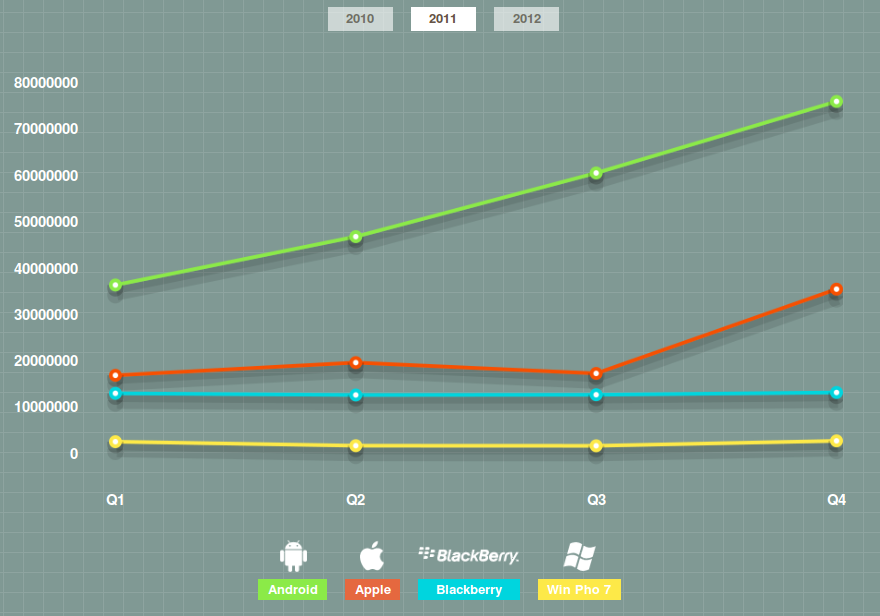
\includegraphics[width=0.8\textwidth]{figures/sales_2011}
	\caption{Čtvrtletní prodeje zařízení s vybranými operačními systémy v roce 2011 (celosvětově).\protect\cite{mobile_stats}}
	\label{fig:sales_world}
\end{figure}
\begin{figure}[p]\centering
	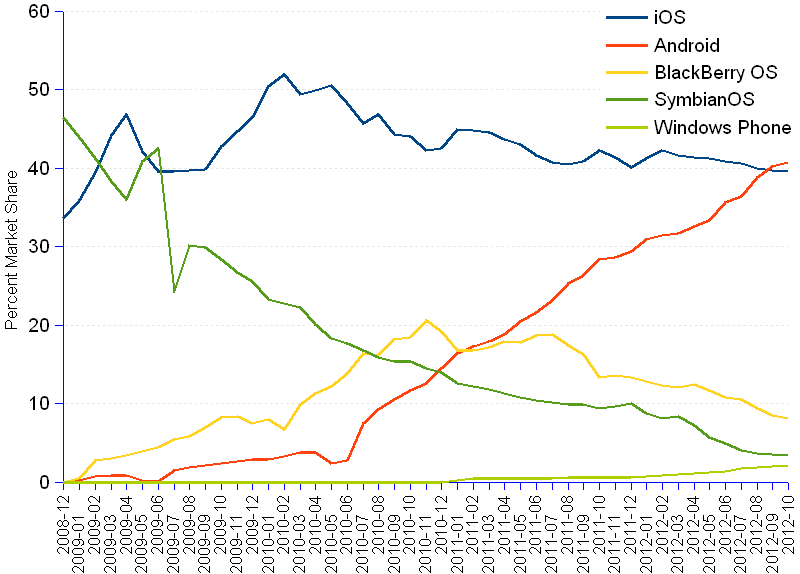
\includegraphics[width=0.8\textwidth]{figures/mobios_eu_timeseries_800x574}
	\caption{Vývoj zastoupení na trhu pro jednotlivé operační systémy v Evropě.\protect\cite{market_share}}
	\label{fig:sales_europe}
\end{figure}

Z uvedených grafů \ref{fig:sales_world} a \ref{fig:sales_europe} na straně \pageref{fig:sales_world} je zřejmé, že hlavními hráči na trhu jsou Apple iOS a Google Android, u kterého je pak rostoucí trend jasně patrný, stejně jako u Windows Phone. Jeho podíl na trhu je sice zatím malý, ale do budoucna se zdá být slibnou platformou. Otázkou je, zda (a případně jak rychle) se mu podaří výrazněji konkurovat ostatním platformám.

Současný trend navíc odhaluje nastávající zlom pro zrakově postižené. Dříve byl pro tuto část trhu jasnou jedničkou operační systém Symbian OS, u kterého ale zřetelně vidíme propadající se tendenci. Tito uživatelé budou v budoucnu nuceni přecházet (pokud již tak neučinili) na jiná zařízení s jinými operačními systémy. Z toho vyplývá že namísto jedné cílové platformy jich tu budeme mít hned několik - nejpravděpodobněji právě ty, které jsou předmětem naší rešerše.

\subsection{Spokojenost uživatelů}
Cílem každé aplikace by měla být maximální spokojenost uživatelů při jejím používání a nejinak je tomu u samotných operačních systémů. Pokud nebude uživatel spokojen s jeho celkovým používáním, bude mít tendence poohlížet se po jiném řešení, kde jinde než u konkurence. Navíc jeho nespokojenost z operačního systému může paušálně ovlivňovat i dojmy ze samotné aplikace.

V rámci každoroční čtenářské ankety \uv{Readers’ Choice Awards} zjišťuje webová stránka pcmag.com celkovou spokojenost uživatelů s používáním operačních systémů na zařízeních, která vlastní a denně používají. Hodnocení zobrazené na grafu \ref{fig:satisfaction} na straně \pageref{fig:satisfaction} probíhá v mnoha kategoriích, např. dostupnost aplikací, hudební přehrávač nebo spolehlivost. Jak vidíme na přiloženém grafu, nejvíce spokojeni jsou uživatelé s Apple iOS a Windows Phone, na třetím místě se se ztrátou 0.8 bodu umístil Google Android.

\begin{figure}[p]\centering
	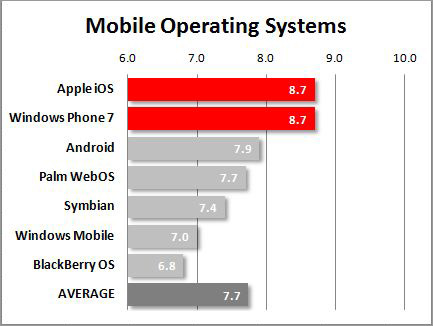
\includegraphics[width=0.8\textwidth]{figures/339723-mobile-operating-systems}
	\caption{Spokojenost uživatelů s jejich operačním systémem (10.0 - nejlepší) vypracovaný webovou stránkou pcmag.com.\protect\cite{pcmag}}
	\label{fig:satisfaction}
\end{figure}
\begin{figure}[p]\centering
	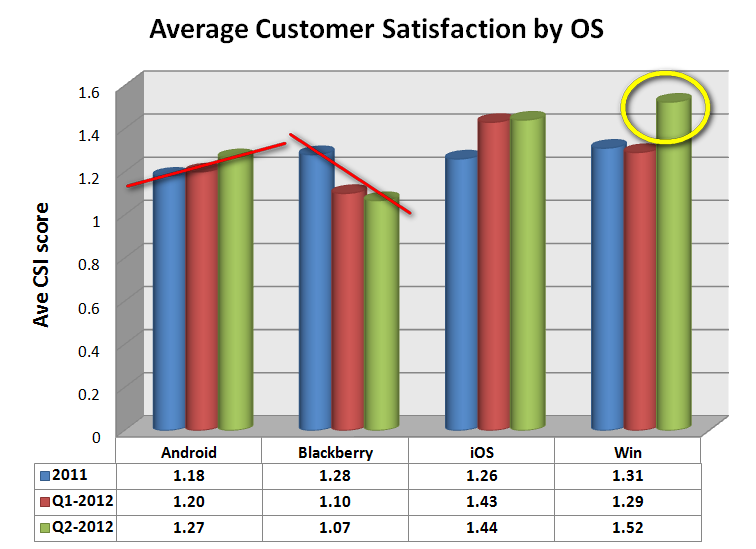
\includegraphics[width=0.8\textwidth]{figures/CSI-by-OS-Q2-12}
	\caption{Přehled průměrné spokojenosti zákazníků s daným operačním systémem vypracovaný v rámci studie Amplified Analytics.\protect\cite{amplified}}
	\label{fig:satisfaction2}
\end{figure}

Jeden z výsledků studie zobrazené na grafu \ref{fig:satisfaction2} na straně \pageref{fig:satisfaction2} potvrzuje rostoucí tendenci spokojenosti u operačního systému Google Android společně s Apple iOS. Windows Phone v posledním zkoumaném období zaznamenal znatelný skok, ale vzhledem k předchozímu vývoji z toho nelze mnoho usuzovat.

Pro komunitu zrakově postižených bohužel žádné takové ankety ani údaje nemáme, proto se o spokojenosti těchto uživatelů můžeme jen domnívat na základě jejich zkušeností, o které se s námi podělili ať už v rámci uživatelského výzkumu nebo článků na internetu.

\subsection{Cena koncových zařízení}
Důležitým kriteriem pro výběr nového telefonu může být pro zákazníka tzv. poměr cena/výkon, tedy co všechno dostane za danou cenu. V případě uvažovaných operačních systémů je zřejmé, že výhodu v tomto ohledu budou mít Google Android a Windows Phone a to především proto, že jsou distribuovány na mnoho koncových zařízení s různými cenami a od různých výrobců. Zákazník tak má díky tomu podstatně širší paletu možností.

Přesným opakem tohoto systému pak je Apple iOS, který je distribuován výhradně na zařízení produkovaná společností Apple, která si samozřejmě určuje i cenu koncových zařízení. Není žádným tajemstvím, že řešení od společnosti Apple v mnoha případech cenově přesahují srovnatelná zařízení s ostatními operačními systémy - což ovšem dohání například nápaditými a inovativními řešeními v oblasti ovladatelnosti a použitelnosti. Koncový zákazník tímto přístupem získá výhodu uniformního prostředí, ovšem na úkor ztráty variability výběru.

Provedeme-li jednoduchý průzkum například v rámci serveru Heureka\cite{heureka}, dojdeme k jasnému závěru. Na spodním konci cenového rozpětí (tedy nejlevnější řešení) se nachází zařízení s operačním systémem Google Android. Pravým opakem jsou pak řešení s operačním systémem Apple iOS, které jsou v současnosti nejdražší.

Trochu jiným pohledem se však musíme podívat na problematiku zrakově postižených, protože u těchto uživatelů může být měřítko cena/výkon určitým způsobem vychýlené díky případné chybějící funkcionalitě. Omezujícím faktorem pak není tolik cena, jako právě (nadstandardní) možnosti zařízení, jejichž absence pro vidícího uživatele žádný problém nepředstavuje. Například se může jednat o hardwarová tlačítka, klávesnici nebo o kvalitu ozvučení systému a jeho ovládání pomocí nadefinovaných gest.

S tím tedy úzce souvisí případná limitace výběru na dražší zařízení a následně dotační politika, na základě které může být zrakově postiženému poskytnuta finanční pomoc. Za jakých podmínek mohou o některou formu příspěvku tito lidé žádat jsme se dozvěděli v odpovědi na náš emailový dotaz od Evy Vonešové z informačního centra Tyflonet (celé znění v příloze \ref{att:tyflonet} na straně \pageref{att:tyflonet}). Protože se s velkou pravděpodobností obvykle jedná o pomůcku do 24 000 Kč, může být taková finanční pomoc poskytnuta pouze osobám se stanovenou výškou příjmu.

\subsection{Dostupné aplikace}
Abychom si udělali ucelený obraz o trhu a jeho vývoji, je vhodné zanést do našeho rozhodování také údaje o dostupných aplikacích pro dané operační systémy. Mělo by nás zajímat, zda počet dostupných aplikací v jednotlivých webových obchodech stoupá nebo stagnuje.

V případě, že daný operační systém zaznamenává rostoucí tendenci, můžeme se domnívat, že ostatní vývojářské firmy stále vidí v této sekci trhu příležitost a především peníze, tedy potencionální zisk. Samozřejmostí je, že tato domněnka platí u stagnujících počtů dostupných aplikací zcela opačně. Tento fakt může především znamenat, že operační systém přestává být pro vývojáře perspektivní nebo může svědčit o aktuálním nasycení trhu.

Na grafu \ref{fig:apps} na straně \pageref{fig:apps} si můžeme povšimnout viditelně stoupající tendence u všech námi vybraných operačních systémů. Jasně se ale potvrzuje prozatímní dominantní postavení Google Android a Apple iOS, kteří nabízeli v Q2 2012 500000 a 650000 aplikací, přičemž v grafu vidíme, že prvně jmenovaný svého hlavního konkurenta začíná dohánět. Zároveň nás také zaujme vývoj počtu dostupných aplikací u operačního systému Windows Phone, což naznačuje jeho stoupající oblíbenost jak mezi uživateli, tak mezi vývojáři.

\begin{figure}\centering
	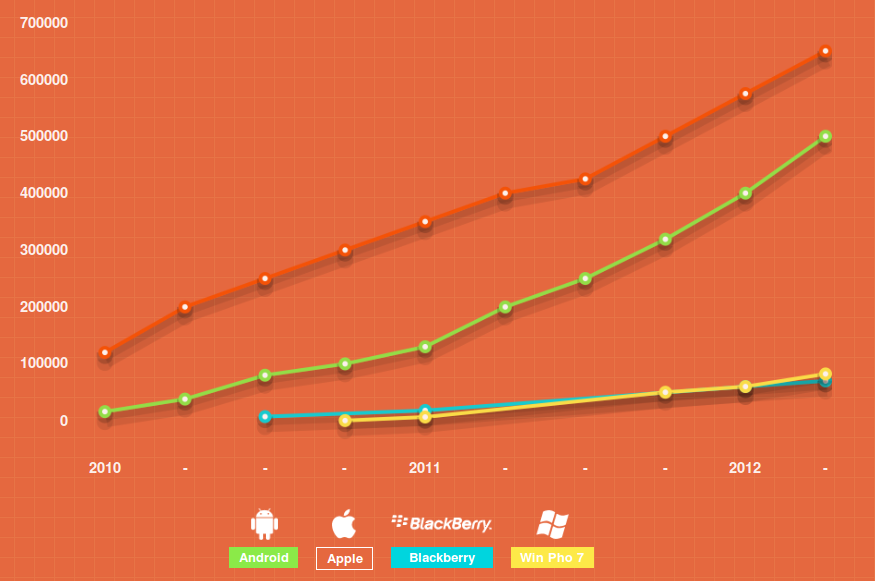
\includegraphics[width=0.8\textwidth]{figures/apps_available}
	\caption{Vývoj počtu dostupných aplikací pro jednotlivé operační systémy.\cite{mobile_stats}}
	\label{fig:apps}
\end{figure}

Měli bychom ale zároveň mít na paměti, že vysoké množství dostupných aplikací nutně nemusí garantovat jejich kvalitu ani použitelnost. V otázce kvality pak záleží na tom, jakou politiku v tomto směru vyznává daná společnost. Například aplikace publikovaná na Apple App Store by měla procházet oproti Google Play, kde je publikování volnejší, před svým uveřejněním poměrně složitým schvalovacím procesem. Na druhou stranu, přítomnost více aplikací poskytujících podobnou funkcionalitu dává uživatelům větší volnost a možnost vybrat si tu, která jim nejvíce vyhovuje.

Problém s relevantností tohoto kritéria může nastat v případě zrakově postižených. Z dostupných zdrojů nejsme schopni žádným způsobem usoudit, kolik z těchto aplikací je skutečně vhodných a užitečných pro tuto skupinu uživatelů (především z hlediska přístupnosti). Abychom si mohli alespoň částečně udělat představu o aspektech tohoto problému, bylo by vhodné vybrat několik zástupců z aplikací, které by mohly být pontecionálně zajímavé pro zrakově postižené, a podívat se, jak a zda tyto parametry splňují.

Vhodným nasměrováním při jejich výběru by mohl být uživatelský výzkum a na jeho základě vystavěný vzorový scénář. Pro potřebu porovnání jsme tedy vybrali aplikace z několika oblastí, přičemž se konkrétně jedná o emailového klienta, poslech rádia, mapy, kalendář, vyhledávání spojů MHD, VoIP (Skype), televizní zpravodajství (ČT24), internetový prohlížeč, počasí, poznámky a čtečku knih.

Apple iOS je na zrakově postižené uživatele dobře připraven a aplikace, které jsou nativně zahrnuty v rámci tohoto operačního systému\cite{ios_apps}, lze prohlásit za plně přístupné. Ze zbývajícího seznamu se nám přizpůsobené pro tuto skupinu podařilo najít všechny aplikace kromě čtečky knih (jako specializované aplikace) a u aplikace IDOS pro vyhledávání spojů uživatelé zaznamenali problematicky vyřešený našeptávač, který komplikuje práci s aplikací.

Google Android je, stejně jako jeho konkurent, také ozvučen. Zároveň zde opět platí, že aplikace, které jsou v zařízení nativně nainstalovány lze prohlásit za přístupné\cite{pristupnost}\cite{blind_apps}. Z ostatních aplikací se nám podařilo najít všechny kromě čtečky knih (jako specializované aplikace).

Windows Phone v této kapitole zmíníme pouze letmo, protože samotný systém není vůbec ozvučen a z toho důvodu nemůžeme ani hodnotit kvalitu dostupnosti aplikací.

\subsection{Možnosti a omezení}
V závěru naší rešerše se podíváme na jednotlivé operační systémy z pohledu jejich možností a omezení. Tento problém bychom měli uvažovat jak v rovině uživatelské, tak zároveň vývojářské.

Jak jsme si již uvedli, naše aplikace by měla pomáhat mimo jiné uživatelům, kteří mají nějakou formu postižení zraku. Bude nás tedy samozřejmě zajímat, jak jsou schopny jednotlivé operační systémy komunikovat s takto limitovanými uživateli. Jako kritéria jsem vybrali tyto oblasti:
\begin{itemize}
\item    HW tlačítka (jejich počet, hmatnost, namapovaná funkcionalita)
\item    Ozvučení systému
\item    Accessibility API
\item    Accessibility podpora pro vývoj aplikace + existence a kvalita IDE
\end{itemize}

Hlavním cílem naší aplikace by měla být přímá modifikace výchozího menu operačního systému a nabízení (případně parametrizovaných) aplikací ke spuštení. Důležité je také propojení naší aplikace s funkcemi telefonu. Z vývojářského hlediska nás tedy zajímá, zda se dá něco takového v rámci dané platformy provést či nikoliv, případně za jakých podmínek a co je k tomu nutné. Jako kritéria jsme zvolili tyto oblasti:

\begin{itemize}
\item    Nahrazení/modifikace launcheru
\item    Parametrizované spouštění aplikací
\item    Propojení se základními funkcemi (telefonování, zprávy, kalendář, atd.)
\end{itemize}

\subsubsection{HW tlačítka}
Operační systém Apple iOS se vyskytuje (jak jsme si uvedli již dříve) na omezeném množství zařízení. Tím pádem máme celkem přehled o designu všech modelů a také o výhledu do budoucna. V současné době je vzhled jednotlivých zařízení unifikovaný a politika společnosti Apple nenaznačuje, že by se mělo něco radikálně měnit (není tedy pravděpodobné, že by například začala vyrábět zařízení s HW klávesnicí).

Na těle iPhone najdeme celkem 4 fyzická tlačítka (přední strana - tlačítko Home (Domů), levá strana - dvě tlačítka pro ovládání hlasitosti, horní strana - uspávací/vypínací tlačítko) a jeden přepínač (levá strana - dvoupolohový přepínač tichého a hlasitého módu)\cite{iphone}. Hmatnost všech tlačítek a přepínače je zřejmá hned na první pohled a neměl by s ní být žádný problém. Všechny ovládací prvky buď vystupují nebo vytvářejí prohlubeň (tlačítko Home) a mají zároveň jasně namapovanou funkcionalitu\cite{iphone_anatomy}. Tento fakt ovšem nebrání vývojářům si chování některých prvků přemapovat (například aplikace pro fotografování může fotit stiskem tlačítka pro ovládání hlasitosti), ačkoliv je to striktně proti politice společnosti Apple.

Situace operačního systému Google Android bude přesně opačná. Vzhledem k tomu, že je prodáván na velmi mnoha různých zařízeních je prakticky nemožné najít jakýkoliv unifikovaný design. Pro tato zařízení bývají typická tlačítka pro ovládání hlasitosti (obvykle na boku) a pro uspání/vypnutí (nahoře), s jejichž hmatností by neměl být problém. Pod displayem obvykle najdeme v dolní části 3 ovládací prvky (u některých zařízení ovšem i 4), přičemž u starších zařízení se mohlo jednat i o trackball nebo trackpad. Hmatnost těchto prvků přitom není u novějších zařízení příliš dobrá, protože nijak nevystupují (až na výjimky v podobě některých výrobců, kteří ponechávají vystupující Home tlačítko) a v některých případech se v podstatě nejedná ani o HW tlačítka v pravém slova smyslu. Jejich výhodou je, že poskytují zpětnou vazbu ve formě zavibrování. Některá zařízení navíc disponují HW vysouvací klávesnicí - zde je hmatnost kláves samozřejmě v pořádku.

Všechny prvky mají pevně danou funkcionalitu, ovšem problém může nastat napříč různými výrobci v případě prvků pod displayem. Neexistuje totiž jednotný postup pro mapování určité funkcionality na určitý prvek. Může se tak stát, že například tlačítko pro funkci “zpět” bude u jednoho výrobce vpravo a u druhého vlevo. V zásadě však platí, že se na těchto pozicích vždy nachází prvky se stejnou funkcionalitou, jenom jinak uspořádané. I v tomto případě je možné přemapovat chování některých prvků a i v tomto případě to není doporučeno ze strany společnosti Google.

Windows Phone na tom je podobně jako Google Android. Necílí primárně na jeden typ zařízení a proto dochází k tomu, že se s ním můžeme setkat u více výrobců (prozatím pouze HTC a Nokia). Nicméně se zdá, že si oproti zařízením s výše zmíněným operačním systémem zachovávají jednotné rozložení prvků pod displayem. V ostatních oblastech se prakticky shodují.

\subsubsection{Ozvučení systému}
Z našich uživatelských testů a dostupných článků\cite{ipad_blind}\cite{iphone_blind}\cite{iphone_inside} vyplývá, že Apple iOS nabízí svým zrakově postiženým uživatelům vysoký komfort použitelnosti. Ti mohou aktivovat režim zpřístupnění zcela bez pomoci vidící osoby.

Google Android je na tom oproti konkurentovi z předchozího odstavce hůře (verze 2.3.x), i když po jistých úprávách zařízení (které však, narozdíl od Apple iOS, zrakově postižený uživatel sám nezvládne) lze docílit poměrně uspokojivé formy přístupnosti\cite{android_blind}. Na zvýšení tohoto komfortu navíc Google zapracoval a k jeho podstatnému zlepšení dochází s verzí 4.0, která už se velmi přibližuje úrovni, kterou nabízí Apple iOS\cite{android_start}.

Windows Phone si ze všech našich zkoumaných operačních systémů vede patrně nejhůře, což také dokazují mnohé články\cite{touch_yes_or_no}\cite{win8_blind}\cite{win8_blind2} uživatelů zabývající se touto problematikou. Současná situace tedy podle všeho vypadá tak, že pro tuto platformu neexistuje žádný odečítač obrazovky a proto se v současné době jeví jako absolutně nepoužitelná pro uživatele se zrakovým postižením, ačkoliv si firma Microsoft tento fakt zjevně uvědomuje a některé mírné formy zrakového postižení reflektovala v nastavení přístupnosti\cite{win8_no_reader} (které však pro nás prozatím nejsou dostačující). Toto zjištění může být obzvláště nepříjemné pro uživatele předchozího operačního systému od Microsoftu - Windows Mobile. Ten totiž s přístupností problémy neměl a pokud budou chtít přecházet na jeho nástupce, bude to pro ně v současné chvíli znamenat neřešitelný problém.

\subsubsection{Accessibility API}
Apple iOS na svých stránkách pro vývojáře poskytuje detailní informace k problematice přístupnosti pro zrakově postižené\cite{iphone_blind_dev}. Vývojáři jsou předloženy důvody, které by ho měly vést k uvedení těchto principů do praxe a následně zmíněn stručný přehled toho, co může vývojář při svém snažení využít, aby byl finální produkt co nejpřívětivější, v kapitole příznačně nazvané \uv{iPhone Accessibility API and Tools}.

Dokument zabývající se touto problematikou v rámci platformy Google Android poskytuje svým vývojářům prakticky stejné informace jako operační systém zmíněný v prvním odstavci. Za zmíňku jistě stojí kapitola \uv{Accessibility Developer Checklist}, poskytující vývojářům seznam bodů, na základě kterých se ujistí, že je jejich aplikace plně přístupná zrakově postiženým uživatelům.

Vzhledem k celkové absenci odečítače obrazovky na platformě Windows Phone nemůžeme očekávat žádná doporučení a pokyny pro vývoj aplikací dostupných zrakově postiženým uživatelům.

\subsubsection{Vývoj aplikací}
Apple nabízí svým vývojářům návody, jak a proč svou aplikaci udělat přístupnou uživatelům se zrakovým postižením\cite{iphone_blind_dev}. Na problém ovšem narazíme v případě, že se začneme zajímat o způsob, jak aplikace pro Apple iOS vyvíjet. Zjistíme totiž, že budeme potřebovat vývojové prostředí (IDE) nazvané Xcode ve spojení iOS SDK, které je zdarma, ovšem dostupné pouze pro operační systém OS X, což ve spojení s adekvátním hardwarem znamená nezanedbatelné výdaje.

Google v tomto případě samozřejmě nijak nezaostává a svým vývojářům také nabízí oficiální návody, jak zpřístupnit své aplikace zrakově postiženým\cite{android_blind_dev}. Získává ovšem navrch v případě volby vývojového prostředí. Oficiálně podporované je Eclipse IDE s Android SDK, které je multiplatformní\cite{cross_platform} (v současné době dostupné pro Linux, Windows a Mac OS X) a zdarma. Pro ty, kteří z nějakého důvodu nechtějí využívat služeb Eclipse IDE, jsou na oficiálních stránkách pro vývojáře\cite{android_dev} připraveny návody, jak vyvíjet aplikace pomocí jakéhokoliv jiného prostředí.

Vzhledem k tomu, že Windows Phone zatím žádnou větší podporu přístupnosti pro zrakově postižené nenabízí, nedá se ani očekávat, že by pro své vývojáře nabízel doporučení nebo ucelený pohled na tuto problematiku. Pro vývoj aplikací na Windows Phone je zapotřebí stáhnout Windows Phone SDK\cite{win_sdk}, které v sobě obsahuje všechny potřebné nástroje\cite{win8_sdk} (především Microsoft Visual Studio). Krokem kupředu je uvolnění jejich speciálních verzí zcela zdarma, nicméně faktem zůstavá, že k plnohodnotnému vývoji aplikací bude zapotřebí operační systém Microsoft Windows. V případě SDK pro Windows Phone 7.x to jsou Windows 7 / Windows 8 / Windows 8 Pro / Windows Vista, pro Windows Phone 8 pak dochází k zeštíhlení pouze na Windows 8 / Windows 8 Pro.

\subsubsection{Nahrazení/modifikace launcheru}
V současné chvíli není v případě Apple iOS legálně možné modifikovat launcher (Home screen) jako celek. Existují sice aplikace, které určitým způsobem umožňují jeho modifikaci\cite{iphone_shortcuts}, to nám však pro naše účely nestačí. Nahrazení stávajícího launcheru tedy není možné bez operace nazývané jailbreak\cite{ios_jailbreak}, která je ovšem porušením licenční smlouvy koncového uživatele\cite{apple_about_jailbreak}. Po jejím provedení je na toto zařízení možné nahrávat neoficiální aplikace a tím pádem i aplikaci umožňující změnu standardního launcheru\cite{iphone_launcher}.

Naproti tomu Google Android nemá s touto operací žádný problém, jelikož se u něj jedná o nahrazení stávající aplikace (launcheru) aplikací jinou (podobně jako nahrazení standardní klávesnice, emailového klienta atp.) bez jakékoliv jiné úpravy telefonu. Dokonce existuje zdrojový kód standardního launcheru ke stažení a inspiraci\cite{android_launcher} a stejně tak mnoho jiných vývojářských počinů (například ADW Launcher\cite{android_adw_launcher}).

Windows Phone vyznává z hlediska vývoje u svého launcheru (Start screen) podobnou myšlenku jako Google Android, nicméně vzhled je naprosto rozdílný. Zdá se však, že požadovaná modifikace launcheru je v zásadě možná, vzhledem k dostupným aplikacím na Windows Phone Marketplace, které řeší podobný problém\cite{win_launcher}\cite{win_launcher2}.

\subsubsection{Parametrizované spouštění aplikací}
Podstatnou úsporou času by mohla být pro uživatele situace, kdy jedním kliknutím spustí aplikaci, které bude při jejím spuštění předán jeden nebo více parametrů. V ideálním případě by tím pádem mohl náš launcher ušetřit uživateli čas, který by strávil v rámci ruční konfigurace, a zjednodušit interakci. Například přehrávači rádií by tak mohla být předána konkrétní stanice, vyhledávači spojení start a cíl nebo aplikaci Skype indetifikátor uživatele.

Apple iOS umožňuje toto realizovat pomocí tzv. URL Scheme\cite{apple_url_scheme}, pomocí kterého se aplikace v operačním systému registrují pro využití ostatními\cite{apple_app_launch} a předat jim parameter\cite{apple_app_launch2}. Podobný postup lze uplatnit také v případě operačního systému Google Android v podobě intentů\cite{android_app_launch}. Windows Phone nabízí podobnou možnost jako oba zmíněné operační systémy v rámci tzv. protocol handlers\cite{win_app_launch}.

Omezujícím faktorem samozřejmě zůstává, že aplikace, které hodláme spouštět, musí tuto funkcionalitu podporovat a korektně se registrovat v rámci operačního systému.

\subsubsection{Propojení se základními funkcemi}
Apple iOS umožňuje vývojáři komunikovat s vestavěným kalendářem a dokonce se registrovat pro přijímání upozornění o změnách\cite{apple_listener}. Nepodařil se nám však dohledat přehled všech možných notifikací, ke kterým se lze v rámci naší aplikace přihlásit. Pravděpodobně to však nebude možné u aplikací spravujících telefonní hovory, textové zprávy nebo emaily, jelikož iOS oficiálně neumožňuje přistupovat k jejich záznamům v logu\cite{apple_history}. Podobně se nám nepodařilo dohledat informace o možném přístupu k nastavení systému (GPS, Wi-Fi atp.).

Google Android také umožňuje komunikaci s vestavěným kalendářem\cite{android_calendar}\cite{android_calendar2}, nicméně registrace pro přijímání upozornění o změnách není příliš komfortní\cite{android_calendar3}\cite{android_calendar4}. Oproti operačnímu systému Apple iOS však vývojáři nabízí přístup k záznamům telefonních hovorů\cite{android_calllog} a neoficiálně i k textovým zprávám, nicméně se jedná o obecně nedoporučovaný způsob, který nemusí zaručovat potřebnou funkcionalitu na všech zařízeních\cite{android_sms} a podobná situace pravděpodobně nastane v případě emailových zpráv. Požadovaného chování vzhledem k zachytávání upozornění o změnách objektů bychom však mohli dosáhnout pomocí tzv. ContentObserverů\cite{android_observer}. Systémové nastavení, například stav přijímače GPS\cite{android_gps}, Wi-Fi\cite{android_wifi} nebo zvukový profil\cite{android_profile}, se dá jednoduše zjistit.

Windows Phone, stejně jako jeho konkurenti, rovněž nabízí přístup k datům kalendáře\cite{win_calendar}, ale možnost registrovat se k pozorování změn se nám nalézt nepodařilo. Stejná filosofie jako v případě operačního systému Apple iOS je zde pak uplatňována v případě přístupu k seznamu hovorů a textových zpráv\cite{win_incoming_event}. Podobně jako u platformy Google Android je i zde možné získat informace o GPS\cite{win_location} a Wi-Fi\cite{win_wifi}.

\subsection{Výsledky řešerše}
Ze průzkumu provedeném v předchozích kapitolách bychom měli být nyní schopni vybrat mobilní operační systém, který se pro naše potřeby hodí nejvíce. Jak se ukázalo, naprosto nevhodný je v současné chvíli operační systém Windows Phone z důvodu absence odečítače obrazovky a prakticky nulové podpory pro uživatele se zrakovým postižením stejně jako vývojářů zaměřených na tuto skupinu.

Operační systémy Apple iOS a Google Android jsou velmi vyrovnanými soupeři a rozhodovat mezi nimi tedy budeme na základě specifických kritérií. Apple iOS a jeho zařízení jsou vhodnější pro nevidomé uživatele z pohledu uniformního prostředí, nicméně Google Android jasně vyhrává v pro nás důležitých oblastech, kterými jsou snadná modifikace launcheru a multiplatformní IDE, které díky tomu nevyžaduje externí náklady v podobě zakoupení licence opračního systému (lze vyvíjet i na Linuxu). Neméně důležitá je i oficiální možnost přístupu k informacím o stavu mobilního zařízení.

Na základě výše uvedených argumentů budeme pro následný vývoj naší aplikace favorizovat právě operační systém Google Android.

\section{Sémantický model}\label{sec:semantic_model}
Sémantický model si nejlépe popíšeme pomocí diagramu \ref{fig:semantic} na straně \pageref{fig:semantic}, na kterém je znázorněna struktura OWL modelu. V něm se vyskytují třídy (zvýrazněny tučně), jejich instance (ostatní) a vztahové relace (plná šipka - dědičnost, čárkovaná šipka - vztah) a je rozdělen na tři části - první popisuje třídy a jejich instance, které jsou pro naši aplikaci pevně stanoveny a v současném stavu se nepočítá s jejich modifikací.

\begin{figure}\centering
	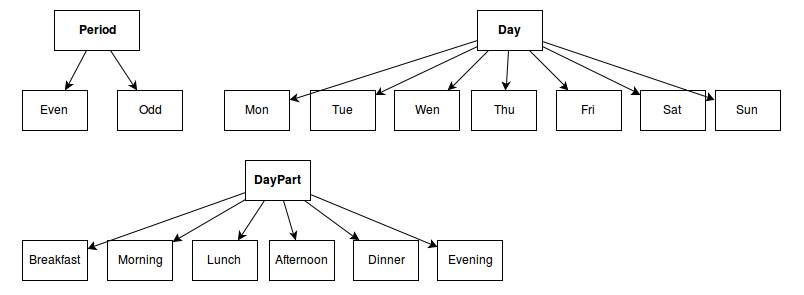
\includegraphics[width=1\textwidth]{figures/semantic1}
	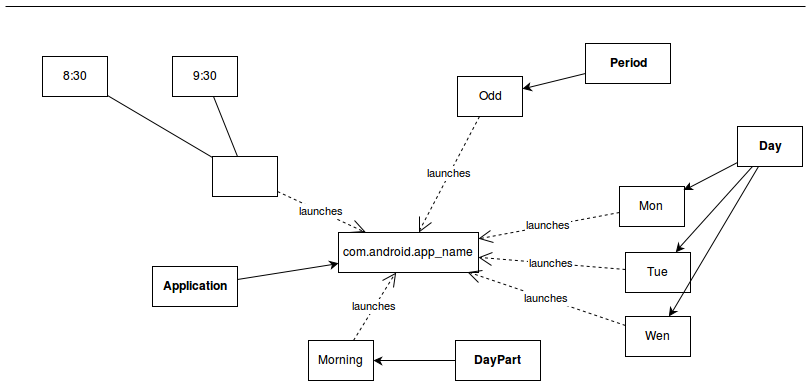
\includegraphics[width=1\textwidth]{figures/semantic2}
	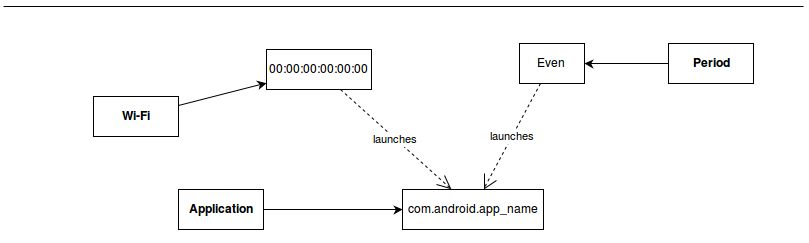
\includegraphics[width=1\textwidth]{figures/semantic3}
	\caption{Sémantický model.}
	\label{fig:semantic}
\end{figure}

Druhá část už popisuje konkrétní strukturu uložené pravidelné aktivity a je na ní vidět její typ (com.android.app\_name) a události, které ji spouštějí - dny v týdnu, časové období, část dne a týdenní perioda. Třetí část se pak zabývá odlišnou strukturou, kdy spouštění aplikace obvykle probíhá v době, kdy je zařízení připojeno ke specifické Wi-Fi a to vždy v lichém týdnu.

Protože bychom v rámci našeho projektu naplno nevyužili všech možností, které OWL model nabízí, a zároveň se obáváme zbytečného nárůstu výpočetních prostředků vzhledem ke komplexnosti a velikosti dostupných reasonerů, které navíc nejsou optimalizovány pro mobilní zařízení, jsme se proto rozhodli převést ho na model v rámci relační databáze. Jednotlivé tabulky budou podrobně rozvedeny v kapitole \ref{sec:er_model} na straně \pageref{sec:er_model}.

\subsection{Period}
Z provedených uživatelských rozhovorů vyplývá, že drtivá většina participantů má pravidelný týdenní cyklus. V rámci dosažení univerzálnější použitelnosti naší aplikace jsme se však rozhodli brát v potaz cyklus čtrnáctidenní vzhledem k tomu, že se v životě velké části populace kdekoliv na světě velmi často vyskytuje. Studenti se s tímto systémem sudých/lichých týdnů setkávají již od základní školy. Tomu se navíc, především v nižších ročnících, obvykle přizpůsobují i dospělí. Naplno pak dochází k jeho uplatnění při studiu na vysokých školách nebo v rámci pracovní doby zvané \uv{krátký, dlouhý týden}.

Tato třída tedy bude obsahovat dvě pevně stanovené hodnoty Even (sudý) a Odd (lichý).

\subsection{Day}
Třída reprezentující jednotlivé dny v týdnu s neměnými hodnotami Mon (Monday - pondělí), Tue (Tuesday - úterý), Wen (Wednesday - středa), Thu (Thursday - čtvrtek), Fri (Friday - pátek), Sat (Saturday - sobota) a Sun (Sunday - neděle).

\subsection{DayPart}
Při stanovení pevného rozložení dne do několika stanovených částí jsme vycházeli z běžného rozdělení tak, jak ho zná drtivá většina uživatelů na celém světě. Námi zvolený cyklus dne začíná hodnotou Breakfast (snídaně), následuje Morning (dopoledne), Lunch (oběd), Afternoon (odpoledne), Dinner (večeře) a končí Evening (večer). Tyto údaje nebude schopna naše aplikace zjistit jiným způsobem, než přímou interakcí s uživatelem. Budeme se tedy muset o těchto hodnotách informovat a zároveň zajistit, aby se tento postup pro něj nestal kontraproduktivním.

\section{Model datového skladu (ER model)}\label{sec:er_model}
Pro persistentní ukládání dat bude v rámci naší aplikace ideální využití některého z dostupných databázových strojů. Model datového skladu slouží k vytvoření abstraktního popisu databázové struktury a vztahů mezi jednotlivými entitami v ní uložených. Díky tomu je zaručena variabilita a možnost volby konkrétního stroje až ve fázi implementace.

Entitu si můžeme představit jako určitou abstrakci nad všemi konkrétními záznamy dané tabulky, můžeme ji tedy tzv. \uv{instanciovat} (naplnit ji) jakýmkoliv záznamem v tabulce. Název jednotlivých tabulek je vždy reprezentován názvem entity v jednotném čísle. V rámci jedné tabulky sice bude postupem času přibývat jednotlivých záznamů a mohlo by se tedy spíše nabízet pojmenování tabulky množným číslem, avšak každý záznam (tedy řádek) v tabulce reprezentuje pouze jednu instanci dané entity. Pomocí unikátního indetifikátoru si tedy saháme právě na ni.

Druhým důvodem pro toto řešení je, že tabulky bývají často v aplikaci mapovány na jednotlivé modely (tedy třídy, reprezentující entity pro potřeby aplikace) pomocí takzvaného ORM. V tomto případě pak tato třída tvoří analogii s entitou v databázi a reprezentuje abstrakci ve formě výše uvedené třídy programovacího jazyka.

Diagram modelu datového skladu\ref{fig:er_model} na straně \pageref{fig:er_model}, metodiku jeho plnění a strukturu jednotlivých tabulek si dále blíže popíšeme v následujících kapitolách.

\begin{figure}\centering
	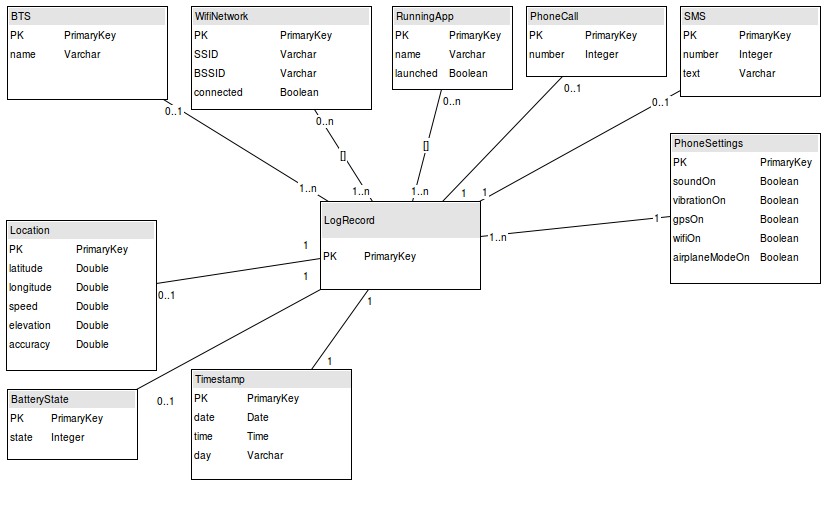
\includegraphics[width=1\textwidth]{figures/er_model1}
	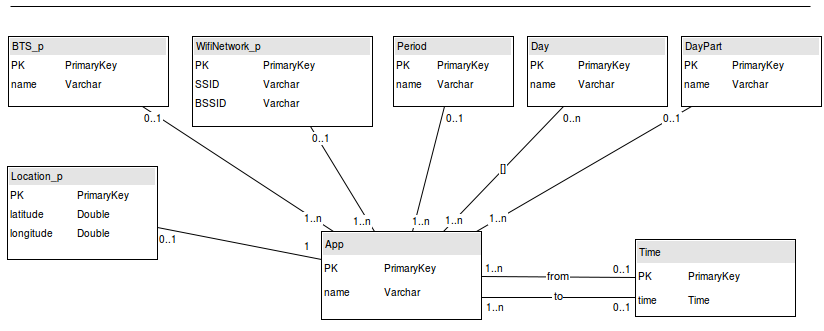
\includegraphics[width=1\textwidth]{figures/er_model2}
	\caption{Model datového skladu (ER model).}
	\label{fig:er_model}
\end{figure}

\subsection{Plnění a správa datového skladu}
Primárním úkolem našeho datového skladu bude uchovávání informací o uživatelských akcích (tedy něco velmi podobného systémovému logu - aktuální snímek stavu telefonu a operačního systému). Důležité je si uvědomit, že pokud se rozhodneme vytvořit nový logovací záznam, budou do databáze uloženy všechny atributy, které sledujeme (neuloží se tedy pouze poloha, ale i okolní Wi-Fi, spuštěné aplikace atp.). Předpokladem této práce je, že se v těchto datech budou nacházet vzory a opakující se aktivity, na jejichž základě se bude naše aplikace schopna dále učit. Algoritmus učení v sobě bude zahrnovat vyhledání těchto pravidelností a jejich následné vyexportování do připravených tabulek, aby s nimi interpretační vrstva mohla pohodlně pracovat.

Při plnění a správě databáze registrujeme několik problematických oblastí, pro které je potřeba najít vhodné řešení tak, aby měl výsledný produkt co nejlepší vlastnosti a univerzální chování.

\subsubsection*{Dvojitý původ dat}
Data, která budeme schraňovat pro pozdější zpracování budou pocházet ze dvou typově rozdílných zdrojů. Některá budou z podstaty věci o své změně dávat vědět sama (změna polohy), u ostatních musíme jejich zaznamenání řídit sami v pravidelných intervalech (seznam běžících aplikací). Na první pohled se zdá, že by se mělo jednat o dva různé algoritmy.

Tomuto implementačnímu pojetí se ve skutečnosti velmi pravděpodobně nevyhneme, nicméně tento postup by v důsledku vedl k jejich vzájemné kolizi v případě, že měnící se poloha by inicializovala ukládání do databáze stejně jako pravidelný časovač. Toto chování by samotné samozřejmě nevedlo k chybě aplikace, je ale nežádoucí vzhledem k tomu, že by docházelo k opakovanému záznamu identické informace a tím zbytečnému zahlcování databáze.

Proto bude nutné oba algoritmy určitým způsobem sjednotit pod nějaký nadřízený prvek, který bude nad jejich součinností dohlížet a efektivně usměrňovat jejich fungování. V současné chvíli se jeví jako nejlepší takové řešení, že bude časovač nastaven na konstantní hodnotu a postupně odkládán, pokud dostatečný přísun informací z prvního typu zdroje zaručí uspokojivé plnění databáze daty.

Během implementace plnění databáze pomocí výše zmíněného časovače bude nutné se vypořádat s případem, kdy nedochází k činnosti ze strany uživatele. Jedná se především o dobu spánku, ale tento problém se dá zobecnit na všechny případy, kdy není mobilní zařízení aktivně využíváno. Vezmeme-li v úvahu dobu, kdy průměrný uživatel spí, jedná se obvykle zhruba až o jednu třetinu dne (myšleno dvacetičtyřhodinový cyklus). Pokud bychom se tímto nezabývali, ukládali bychom do databáze relativně velké množství dat zcela zbytečně.

Při plnění databáze by tedy bylo vhodné reflektovat stav předchozího záznamu. Jestliže se liší jen nepatrně, není zapotřebí provádět nový záznam. Definici míry diference bude teprve potřeba stanovit, pro začátek může být triviálním nastavením rozdílný čas - tedy pokud se aktuálně ukládaný a nejnovější uložený záznam liší pouze v čase, není potřeba nový vytvářet.

\subsubsection*{Redundance dat}
Při plnění databáze se zcela jistě setkáme s jevem, kdy bude během vytváření nových logovacích záznamů jedna (či více) hodnot konstantních v čase. Bude se například měnit poloha, ale zvukový profil nebo stav GPS přijímače bude stále stejný. Pokud bychom v takovém případě ukládali veškeré informace, bude naše databáze zbytečně zahlcována redundantními daty. Proto bychom se v této kapitole měli zamyslet nad tím, zda dokážeme vymyslet nějaké efektivní řešení tohoto problému, případně zda takové vůbec existuje.

Jeden způsob, který se nabízí, je zaznamenávat pouze změny hodnot. Pokud by se tedy měnila poloha, ale zvukový profil by byl ve všech případech stejný, došlo by k zaznamenání této informace (zvukového profilu) pouze v případě zjištění, že byl telefon přepnut do jiného režimu. V ostatních případech by tento údaj vůbec nebyl přítomen a nepřímo by tak odkazoval na starší záznam (nejbližší změnu v minulosti). Zřejmou výhodou je odbourání zátěže databáze neměnícími se daty, která by se tím pádem vůbec neukládala. Naproti tomu je ovšem nevýhodou snížení dostupnosti informací. Pokud bychom si chtěli zjistit stav mobilního zařízení třeba pro určitý den a hodinu, bylo by nutné (v rámci vybraného záznamu) hledat pro všechny nepřítomné hodnoty jejich poslední změny v minulosti, což by ve výsledku mohlo značně zvýšit komplikovanost a snížit rychlost a flexibilitu takových operací.

Další možností by bylo pojmout uspořádání databáze řekněme klasickým relačním způsobem. V rámci každé tabulky by tedy byly uloženy pouze známé (v minulosti zaznamenané) hodnoty a každý nový logovací záznam by obsahoval odkazy na ty, které by v danou chvíli odpovídaly aktuálnímu stavu zařízení (v případě, že by požadovanou hodnotu algoritmus v databázi nenašel, vytvořil by pro ni nový záznam). Tento postup by měl ve výsledku mnoho výhod. Pokud zjišťujeme stav mobilního zařízení pro určitý den a hodinu, máme okamžitě po ruce všechny informace, které si pro tyto účely do databáze ukládáme. V případě, že bychom si chtěli zjistit, kdy a za jakých hodnot je prováděno například spouštění určité aplikace, nám toto uspořádání, oproti možnosti z předchozího odstavce, celý proces usnadní (a obdobně pro ostatní sledované hodnoty). Nevýhodou tohoto řešení bude naopak nutnost u některých vazeb zavést určité \uv{spojovací} tabulky (tedy vzroste objem ukládaných dat), které budou udržovat informace o tom, jaké hodnoty byly uloženy ke konkrétnímu záznamu (v grafu nejsou znázorněny). To by však ve spojení s efektivním čištěním databáze nemělo představovat fatální problém.

Protože preferujeme přístup k informacím v databázi právě prostřednictvím klasického relačního způsobu a vzhledem k obavám z nárůstu časové složitosti ve spojení s nutností implementace algoritmu, který by v prvním případě dohledával relevantní informace pro většinu požadovaných záznamů, jsme se rozhodli přiklonit se k druhému řešení.

\subsubsection*{Čištění databáze}
Vzhledem k předpokládanému objemu ukládaných dat je nezbytné vytvořit určitou strategii pro čistění a promazávání databáze. Nesmí se tak ovšem dít na úkor získaných informací - v žádném případě tedy nesmí docházet ke zkreslování pravidelností v důsledku neopatrného promazávání starších dat. Sestrojit algoritmus, který by efektivně prováděl operace zmíněné v úvodní větě, bude jedním z hlavních cílů naší aplikace.

Zjednodušeně by tedy tento algoritmus měl procházet nasbíraná data a hledat v nich vzory a pravidelnosti. Pokud by měl dostatek informací, aby s jistotou mohl prohlásit zkoumanou aktivitu za pravidelnou, mohl by při dalších iteracích postupně začít odmazávat starší (přebytečné) záznamy o této aktivitě a díky tomu tak udržovat databázi v \uv{minimalistickém} stavu. Tím by zmenšil nároky na databázový stroj a zrychlil by případné další dotazy, které by už nemusely procházet víc dat, než je nezbytně nutné.

S přihlédnutím k faktu, že v této fázi stejně budeme hledat pravidelné aktivity, se zdá v současné chvíli jako nejlepší řešení nalezené vzory při této příležitosti rovnou vyexportovat (v kapitole \ref{sec:semantic_model} na straně \pageref{sec:semantic_model} jsme zmínili důvody, které nás vedly k migraci od OWL řešení směrem k relační databázi) a tím dosáhnout efektivnějšího přístupu k nim. Je zcela zřejmé, že takový postup vyžaduje rozšíření naší aplikace o algoritmus, který by procházel již uložené pravidelné aktivity a porovnával je se záznamy v databázi, aby zajistil jejich aktuálnost - tedy že tato aktivita probíhá i nadále. Díky tomu bychom měli být schopni určitým způsobem odmazávat pravidelnosti v databázi, které se nám podařilo tímto procesem přesunout mimo logovací záznamy do speciálních tabulek. Jak efektivní tento způsob bude, záleží především na struktuře a provázanosti jednotlivých pravidelností.

\subsection{Přehled tabulek datového skladu}
Úkolem této kapitoly je popsat jednotlivé tabulky vyskytující se na diagramu datového skladu. U každé z nich se nachází stručný popis a detaily jednotlivých atributů. Samotný graf je rozdělen na dvě části.

\subsubsection*{Logovací informace}
První část grafu popisuje tabulky pro skladování logovacích informací a jejich atributů. Veškeré vazby jsou v zásadě nepovinné, jelikož se u většiny záznamů může stát, že nebude dostupná informace o Wi-Fi, BTS nebo třeba poloze.

\begin{description}
\item[LogRecord]
slouží jako určitá forma středobodu všech logovacích záznamů a je tedy provázaný se všemi tabulkami, které shromažďují informace o uživatelské nebo systémové činnosti. Vždy musí mít vazbu na záznam v tabulce Timestamp, který určuje časovou linearitu. Ostatní vazby jsou nepovinné (tedy k danému času nemusí existovat záznamy v ostatních tabulkách), protože není zaručeno, že tyto informace budou v danou chvíli dostupné. Pokud v následujících kapitolách zmiňujeme sousloví “informace o aktuálních...” máme tím na mysli právě záznamy vztažené k tomuto časovému záznamu.

\item[BTS]
obsahuje informace o BTS, ke které je telefon aktuálně připojen. V případě konkrétního záznamu se uchovává jméno BTS.

\item[WiFiNetwork]
obsahuje informace o aktuálních Wi-Fi sítích dostupných telefonu. V případě konkrétního záznamu se uchovává jméno Wi-Fi sítě a zda je k ní telefon připojen.

\item[RunningApp]
obsahuje informace o aktuálně bežících aplikacích. V případě konkrétního záznamu se uchovává jméno spuštěné aplikace a údaj, zda byla v době jeho pořízení spuštěna či již běžela.

\item[PhoneCall]
obsahuje informace o provedených telefonních hovorech. V případě konkrétního záznamu se uchovává číslo volaného.

\item[SMS]
obsahuje informace o odeslaných textových zprávách. V případě konkrétního záznamu se uchovává telefonní číslo příjemce a text zprávy.

\item[PhoneSettings]
obsahuje informace o aktuálním nastavení telefonu. Jedná se o profil, stav GPS senzoru, WiFi senzoru a Airplane módu. V případě konkrétního záznamu se uchovává, zda je zapnut zvuk a/nebo vibrace a zda jsou senzory zapnuty či nikoliv.

\item[Timestamp]
obsahuje informace o aktuálním času, při kterém je pořízen záznam do tabulky LogRecord. V případě konkrétního záznamu se uchovává datum, čas a název dne.

\item[BatteryState]
obsahuje informace o aktuálním stavu baterie telefonu. V případě konkrétního záznamu se uchovává stav (v procentech).

\item[Location]
obsahuje informace o aktuální geografické poloze telefonu. V případě konkrétního záznamu se uchovává zeměpisná šířka a délka, rychlost, nadmořská výška a přesnost.
\end{description}

\subsubsection*{Pravidelné aktivity}
Druhá část grafu pak popisuje již vyexportované pravidelné aktivity a jejich atributy. Veškeré vazby jsou v zásadě nepovinné, může se stát, že jedinou dohledatelnou pravidelností bude například pouze připojená BTS nebo Wi-Fi.

\begin{description}
\item[App]
obsahuje informace o aplikaci, jejíž spouštění bylo zaznamenáno jako opakující se ve spojení s některým z uchovávaných atributů. Jedná se, podobně jako u tabulky LogRecord, o určitý středobod všech záznamů o pravidelných aktivitách.

\item[BTS\_p]
obsahuje informace o BTS, ke které byl telefon připojen při spouštění dané aplikace. V případě konkrétního záznamu se uchovává její jméno.

\item[WifiNetwork\_p]
obsahuje informace o Wi-Fi, ke které byl telefon připojen nebo která byla dostupná při spouštění dané aplikace. V případě konkrétního záznamu se uchovává její SSID (jméno) a BSSID (identifikátor přístupového bodu).

\item[Period]
obsahuje informace o časové periodě, ve které docházelo k pravidelnému spouštění dané aplikace. V případě konkrétního záznamu se uchovává její jméno.

\item[Day]
obsahuje informace o dnech, ve kterých docházelo k pravidelnému spouštění dané aplikace. V případě konkrétního záznamu se uchovává jeho jméno.

\item[DayPart]
obsahuje informace o části dne, ve které docházelo k pravidelnému spouštění dané aplikace. V případě konkrétního záznamu se uchovává jeho jméno.

\item[Time]
obsahuje informace o čase. Můžeme si zde všimnout dvou vazeb s tabulkou App pojmenovaných “from” a “to”. Tímto způsobem pokrýváme určité časové období, během kterého byla daná aplikace pravidelně spouštěna (nelze se spoléhat na fakt, že uživatel bude spouštět aplikace přesně v pevně daný čas, ale musíme se vyrovnat s jistou flexibilitou). V případě konkrétního záznamu se uchovává časový údaj.

\item[Location\_p]
obsahuje informace o poloze, ve které docházelo k pravidelnému spouštění dané aplikace. V případě konkrétního záznamu se uchovává její zeměpisná šířka a délka. Tento údaj (podobně jako čas) nelze brát dogmaticky, jelikož uživatel nebude stát vždy na tom samém místě, je tedy potřeba v rámci interpretace počítat s jistou, dopředu stanovenou, kruhovou odchylkou.
\end{description}

\section{Správa datových zdrojů}
V případě spravování datových zdrojů jsme se rozhodli pro podobný princip jaký preferuje Google Android například v případě získávání informací o poloze\cite{android_location}. V zásadě se v tomto modelu setkáme se dvěmi součástmi, které si v následujícím textu blíže rozebereme. Kromě toho si detailně popíšeme vzájemnou spolupráci těchto součástí a také vlastnosti, které takto definovaná struktura má.

\subsection{Manager}
Manager (LocationManager\cite{android_location_manager}) je definován jako třída\cite{class} a slouží k poskytování veškerých informací v rámci konkrétního zdroje stejně jako registraci modulů, které chtějí být upozorněny v případě nastalých změn. V našem případě může být celkové pojetí již definovaných Managerů (LocationManager, WifiManager atp.) zbytečně komplikované a naopak některou doplňkovou funkcionalitu nemusí obsahovat. Proto jsme se rozhodli toto rozhraní co nejvíce zjednodušit pomocí TODO (dedicnost, predprvek), což nám omožní i dodatečné úpravy tak, abychom dosáhli požadovaného chování. Aby mohl být vývojáři definovaný modul registrován pro odběr změn, musí splňovat definované požadavky. Zde přichází ke slovu druhá součást a tou je Listener.

\subsection{Listener}
Listener (LocationListener\cite{android_location_listener}) je definován jako interface\cite{interface}, který musí každý modul, usilující o registraci, implementovat. Díky tomu máme jistotu, že jsme nad všemi registrovanými moduly (listenery) schopni zavolat potřebné metody (například metodu spojenou s akcí “nastala změna pozice”). Zároveň tento způsob poskytuje dostatečnou volnost vývojářům, kteří mohou na nastalou situaci reagovat vlastní implementací těchto definovaných metod.

\subsection{Princip}
Proces fungování takového celku si můžeme ilustrovat na zjednodušeném (jedná se o výřez z celkového systému) diagramu \ref{fig:manager_listener} na straně \pageref{fig:manager_listener} (část od vodorovné čáry výše). Vidíme, že prvek LogManager by chtěl být informován o změnách LaunchManageru (uživatelské spouštění aplikací) a TimeManageru (nastavení časovače).

\begin{figure}\centering
	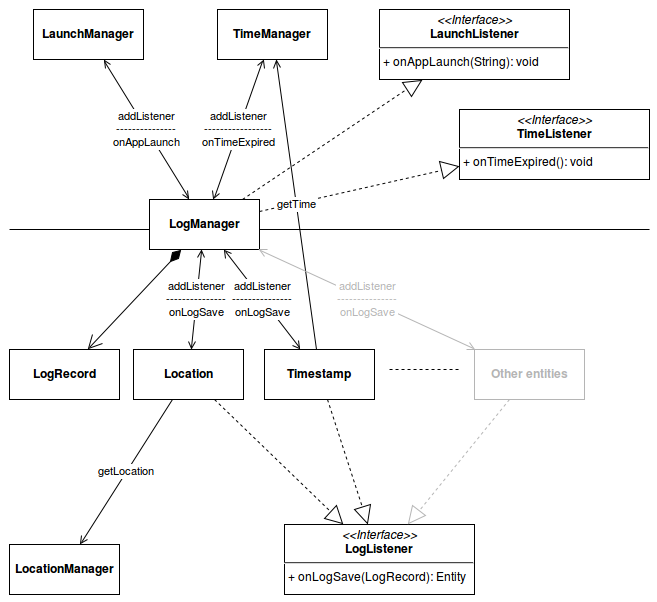
\includegraphics[width=1\textwidth]{figures/manager_listener}
	\caption{Výřez systému ilustrující princip spolupráce součástí Manager a Listener umožňující sledování změn a následné ukládání logovacích záznamů.}
	\label{fig:manager_listener}
\end{figure}

Implementuje proto odpovídající interface (LaunchListener pro LaunchManager a analogicky TimeListener pro TimeManager) a pomocí metody addListener se zaregistruje u každého prvku zvlášť. Ve chvíli, kdy dojde ke sledované změně (spuštění aplikace), LaunchManager projde všechny své LaunchListenery a na nich zavolá definovanou metodu onAppLaunch. LogManager pak na základě toho provede v rámci vlastní implementace této metody odpovídající akci, v tomto případě zarchivuje stav mobilního zařízení (uloží logovací záznam).
Vlastnosti

Takto definovaná struktura nám dává výhodu vzájemné nezávislosti a obstojné flexibility prostřednictvím využití principu registrace Listenerů. Prvky tak mezi sebou nejsou pevně svázány, což nahrává budoucí recyklaci kódu, stejně jako jednoduché rozšiřitelnosti. Díky tomu navíc dosáhneme přehledné správy implementace. U každého modulu je zřejmé, kde může být v současném stavu registrován (vzhledem k uvedenému seznamu implementovaných Listenerů) a Managery zase poskytují přehledně definovaný a jednoduchý přístup k přesně ohraničené části informací (neposkytují zbytečně nic navíc).

Neměl by tak být problém přidat během dalšího vývoje nové Managery a jejich Listenery. Zásah do stávajícího kódu je zřejmý, nicméně popsaný a jasně řízený. Z toho důvodu stačí, když se bude vývojář řídit výše specifikovaným návrhem a dodrží popsanou strukturu.

\section{Ukládání logů}
Požadavkem pro efektivní ukládání logovacích záznamů je dodržení flexibilní a vzájemně nezávislé struktury především z důvodu pravděpodobných změn (rozšíření) během budoucího vývoje. Proto jsme využili mírně upraveného principu popsaného v kapitole [Správa datových zdrojů] (Manager - Listener). V následující kapitole si popíšeme proces jeho fungování a také v čem spočívají drobné modifikace tohoto systému a jaké nás k tomu vedly důvody.

Podíváme-li se na diagram \ref{fig:manager_listener} na straně \pageref{fig:manager_listener}, nejsou zde na první pohled zřejmé žádné procesní změny. Listenery se registrují obvyklým způsobem, mírně rozdílný je však postup při ohlášení změny. LogManager má přímý odkaz na hlavní databázovou entitu LogRecord, která v sobě obsahuje odkazy na mnoho dalších entit, které je potřeba společně uložit do databáze. Aby mohl LogManager entitu LogRecord naplnit, musel by vlastnit odkazy na všechny relevantní entity v databázi. Tento postup by ale odporoval požadavkům na nízkou provázanost a flexibilitu, proto jsme zvolili odlišný algoritmus.

Ve chvíli, kdy LogManager obdrží informaci o změně, vytvoří novou instanci entity LogRecord a tu rozešle všem svým Listenerům (ostatním entitám), kterých v současné chvíli evidujeme dva druhy. První určitým způsobem modifikuje LogRecord a to tak, že mu předá odkaz na svou instanci a LogManageru vrací prázdný odkaz (null). Druhý vytvoří instanci spojovací tabulky (nutné pro vazby many-to-many, například vazba LogRecord - RunningApp), vloží do ní odkaz na obě entity a vrací odkaz na svou vlastní instanci. Neprázdné odkazy si LogManager uchovává a po projití registrovaných Listenerů uloží všechny nashromážděné entity najednou, včetně LogRecordu. Díky tomuto procesu je zaručeno, že do databáze se budou ukládat pouze korektně provázané a úplné záznamy.

Je zřejmé, že než dojde k uložení jednotlivých instanciovaných entit, je potřeba je naplnit relevantními daty. K tomu využijeme již nadefinované moduly z kapitoly [Správa datových zdrojů], které kromě registrace k odběru změn poskytují zároveň přístup k relevantním datům.

\section{Uživatelské rozhraní}
Během implementace našeho projektu se z časových důvodů a vzhledem ke stanoveným cílům nebudeme zabývat hlavní viditelnou součástí, kterou je Launcher. Existuje několik jeho v principu podobných verzí s dostupným zdrojovým kódem, ze kterých vybereme tu nejvhodnější a využijeme ji v našem projektu. Nám tato volba ušetří čas a umožní se soustředit na hlavní cíle projektu, navíc díky tomu bude zaručeno, že nebudeme znovu vynalézat kolo a nutit uživatele zvykat si na něco jiného než co poměrně důvěrně zná a již se s tím naučil pracovat. Jak budeme zobrazovat seznam relevantních aplikací a komunikovat s uživatelem si popíšeme v následujících kapitolách.

\subsection{Seznam aplikací}
Upravovat stávající uživatelské rozhraní tedy budeme pouze minimálně, především z důvodu změny domovské obrazovky, na kterou chceme umístit seznam aplikací. Ten se bude měnit podle toho, jaký bude aktuální kontext, ve kterém se mobilní zařízení (uživatel) nachází, ve spojení s již naučenými pravidelnostmi. Registrujeme několik oblastí, které musíme pokrýt a naplánovat jejich vhodné řešení.

V reakci na měnící se aktuální kontext bude potřeba obnovovat pořadí zobrazených aplikací. Jednou z možností je upravovat seznam aplikací při jakémkoliv vnějším podnětu (změna času, připojení k Wi-Fi). Jeho nevýhodou je ovšem fakt, že by se systém snažil o změnu pořadí i v případě, že uživatel si právě vybírá požadovanou aplikaci. Pokud bychom tuto operaci omezili tím způsobem, aby běžela pouze když je na popředí jiná aplikace, zbytečně bychom mrhali výpočetními zdroji a energií. Tento nedostatek nám však vyřeší způsob, kdy bude k obnovení pořadí docházet v případě, že se naše aplikace vrací na popředí, což umožňuje implementace metody onResume(). Díky tomu budeme kontrolovat aktuálnost pořadí pouze v případě, že se na něj uživatel chystá přejít.

V tomto případě ale může nastat situace, kdy uživatel setrvává na hlavní obrazovce, nicméně nevyvíjí žádnou aktivitu (telefon leží na stole a uživatel nad nečím přemýšlí). V takovém případě by bylo vhodné i přesto, že se naše aplikace nachází v popředí, obnovit pořadí aplikací a nabídnout tak uživateli lepší možnosti vzhledem k aktuálnímu kontextu. Pro vyřešení tohoto problému bude vhodné využít služeb časovače (podobně jako u automatického ukládání logovacích záznamů), který po definované době, během které systém nezaregistruje činnost uživatele, mu pošle zprávu o tom, že má provést revizi stávajícího pořadí.

Tím jsme vyřešili obnovu seznamu aplikací, které ale bude potřeba na hlavní stránce určitým způsobem řadit a toto pořadí se bude měnit v čase. Opět se zde nabízí několik možností, jak přechody mezi jednotlivými stavy vyřešit. Triviálním řešením by bylo se v daném okamžiku podívat, které aplikace je aktuálně relevantní zobrazit, a seřadit je, například abecedně. Vzhledem k tomu, že v současné době nemáme k dispozici žádná data, podle kterých bychom mohli usuzovat na velikost průměrně zobrazovaného seznamu, nelze ani rozumně zhodnotit efektivnost tohoto přístupu.

Sofistikovanějším způsobem řazení by bylo se zaměřit na stanovení priorit, které jednotlivé aplikace v seznamu mají, a na jejich základě v něm pořadí upravovat. Je však nutné nalézt metodu, pomocí které převedeme vlastnosti jednotlivých pravidelných záznamů na jediné číslo - prioritu. Když se na celý problém podíváme detailněji, tak zjistíme, že to není zcela jednoduchá operace. Máme-li aplikaci, která je spouštěna během jednoho dne v týdnu, a druhou, která je spouštěna v přítomnosti specifické Wi-Fi, nejsme v případě, že jsou obě podmínky splněny, schopni určit, která z nich by měla mít prioritu vyšší. Proto se v současné chvíli omezíme na určování priorit pouze u těch aplikací, které mají jasně vymezené časové období (například od 8:00 do 9:00), a ostatním ponecháme tu nejnižší.

\subsection{Komunikace s uživatelem}
Při celkovém pohledu na vyvíjenou aplikaci je zcela zřejmé, že některé informace nejsme schopni zjistit pouze prostřednictvím pasivního sledování uživatelské činnosti. Bez aktivních podnětů tak například těžko zjistíme rozložení dne (jaké časové rozmezí pro uživatele představuje snídaně, dopoledne nebo oběd) nebo jak dané pořadí aplikací odpovídá jeho aktuálním potřebám. Z toho důvodu jsme nuceni nalézt formu, prostřednictvím které budeme s uživatelem komunikovat, tyto informace od něj získávat nebo si nechávat potvrzovat správnost našeho úsudku.

Největším problémem této oblasti je, že se tento způsob shromažďování informací stane pro uživatele otravné nebo ho bude zdržovat při práci. Z jeho pohledu není nic horšího, než když si potřebuje rychle najít spoj a naše aplikace se bude snažit z něj vymámit informace o spokojenosti s aktuálně nabízeným seznamem nebo v jaké se aktuálně nachází fázi dne. Z uvedeného příkladu vyplývá, že si musíme důkladně rozmyslet, kdy budeme po uživateli chtít doplňující informace a když už k tomu dojde, tak především zvolit co nejstručnější formu a dát mu například vybrat z několika nejpravděpodobnějších možností.

Jedním z možných řešení je komunikovat s uživatelem v zásadě pasivně a nechat rozhodnutí, kdy má čas věnovat se zodpovídaní našich dotazů, na něm. Tento způsob by se dal realizovat zobrazením upozornění ve stavové liště, která má ovšem tu nevýhodu, že pro většinu uživatelů může být tato informace obtížně dostupná/zastrčená. Bylo by také nutné shromažďovat více sad dotazů, které bychom pak uživateli předložili a díky tomu by opět mohlo dojít k tomu, že uživatele zahltíme a tím pádem velmi rychle odradíme z důvodu časové zátěže.

Toto provedení pravděpodobně nebude ideální, i když vezmeme v úvahu, že se bude počet dotazů do budoucna pravděpodobně snižovat z důvodu rozsáhlejšího naučení systému. S přihlédnutím k zamýšlené formě sběru informací by bylo vhodnější se ptát po každé provedené operaci. Po spuštění aplikace by se tak uživateli zobrazilo okno s otázkou a po zodpovězení by vše pokračovalo v započatém procesu. Pro zvýšení komfortu by bylo vhodné se uživatele zeptat, zda má v tuto chvíli čas se nám chvíli věnovat. I tak ovšem hrozí, že ho budeme zbytečně zdržovat a proto bychom mohli dotaz raději přesunout na okamžik, kdy se vrací naše aplikace na popředí a je tedy pravděpodobné, že uživatel svou aktuální práci ukončil a mohl by na nás mít více času. V současné chvíli se nám zdá toto řešení jako nejvhodnější.

\chapter{Realizace}
V předešlých kapitolách tohoto dokumentu jsme si definovali čím se bude tato práce zabývat, stanovili jsme si cíle, kterých bychom chtěli dosáhnout, vybrali nejvhodnější platformu, vytvořili návrh a specifikovali řešení nejdůležitějších oblastí, které se budou v naší aplikaci vyskytovat. Nyní se nacházíme ve fázi, kdy přecházíme k samotnému popisu implementace, který by ale nebyl možný bez předchozí práce. Bez důkladně provedeného návrhu řešení a analýzy by tato kapitola byla naprosto bezpředmětná a celkový projekt by mohl snadno skončit zbytečným neúspěchem. 

V této kapitole si přiblížíme některé zajímavé části implementace naší aplikace. Vysvětlíme si strukturu Android projektu tak, jak ho generuje Eclipse IDE. Probereme komunikaci s databází a výběr vhodného Launcheru. Na závěr celé kapitoly si uvedeme, které externí knihovny jsme použili pro řešení typických implementačních problémů.

\section{Adresářová struktura}
Jak nadpis podkapitoly napovídá, popíšeme si zde strukturu Android projektu \cite{android_project_structure} tak, jak je generován při založení nového projektu v Eclipse IDE (obrázek \ref{fig:android_project_structure} na straně \pageref{fig:android_project_structure}).

\begin{figure}
\begin{center}
\begin{verbatim}
.
|-- AndroidManifest.xml
|-- assets
|-- bin
|-- doc
|-- gen
|-- lib
|-- res
|   |-- drawable
|   |-- layout
|   |-- menu
|   |-- values
|-- src
\end{verbatim}
\caption{Adresářová struktura Google Android projektu}
\label{fig:android_project_structure}
\end{center}
\end{figure}

\begin{description}
\item[AndroidManifest.xml] je XML soubor, který uchovává informace o Android aplikaci, jako jsou práva potřebná pro fungování této aplikace (například právo zapisovat na filesystém, právo pro přístup na internet) nebo seznam všech aktivit v systému. Je to zcela nezbytný soubor pro každý Android projekt. Pokud tento soubor chybí nebo je v něm chyba, aplikace se nespustí, popřípadě bude nestabilní.
\item[assets/] má podobný význam jako adresář res, ale zdroje v něm jsou skladovány v \uv{syrovém} stavu a musejí být do aplikace načítány jiným způsobem.
\item[bin/] obsahuje přeložené zdrojové soubory a instalační balíček soardroid.apk
\item[doc/] obsahuje vygenerovanou dokumentaci pomocí nástroje Javadoc
\item[gen/] obsahuje soubor R.java, který je generován automaticky a jsou v něm ukládány odkazy na externí zdroje uložené v res.
\item[lib/] obsahuje .jar soubory externích knihoven použitých v našem projektu, tento adresář není povinný, vytvořili jsme ho pro vlastní potřebu.
\item[res/] je adresář obsahující externí zdroje Android aplikace, které jsou pak přístupné ve zdrojovém kódu díky souboru R.java.
\item[res/drawable] je skladiště obrázků používaných v aplikaci. V některých případech mohou přítomny adresáře s příponou -ldi, -mdi a -hdi, které pak obsahují mutace zdrojů podle rozlišení.
\item[res/layout] obsahuje XML soubory s definicemi šablon pro jednotlivé aktivity. Jeden soubor obsahuje vždy jednu šablonu.
\item[res/menu] obsahuje šablony pro kontextové menu.
\item[res/values] obsahuje XML soubory s texty, barvami atp. Důvodem pro jejich externí skladování je pak snadnější internacionalizace \ref{i18n}.
\item[src/] je poslední a nejdůležitější složka, jsou v ní totiž obsaženy veškeré zdrojové kódy aplikace.
\end{description}

Specifikace a vysvětlení struktury projektu naší aplikace je důležité z hlediska pochopení následujících podkapitol, kde se na některé výše zmíněné adresáře odkazujeme.

\section{Databáze}
Android poskytuje pro potřeby běhu aplikací API pro správu a přístup k databázovému stroji SQLite. Nicméně toto rozhraní se nám, po shlédnutí několika tutoriálů a následném letmém ozkoušení, zdálo přinejmenším zbytečně složité. Co nás v dnešní době velmi překvapilo, je úplná absence nativního přístupu k databázi pomocí ORM. Rozhodli jsme se vyhledat některou alternativu, která by nám tento přístup umožnila. Přímo pro projekty v Androidu se nám podařilo nalézt více knihoven, mezi nimi ActiveRecord\cite{active_record}, OrmLite\cite{ormlite}, ORMDroid\cite{ormdroid} a greenDAO\cite{greendao}. Všechny tyto knihovny zapouzdřují veškerou komunikaci s databází a programátorovi dávájí k dispozici velmi příjemné rozhraní s ORM přístupem k databázi. Pro potřeby naší implementace jsme nakonec zvolili knihovnu ORMDroid ref{ormdroid}, především z důvodu její jednoduchosti a minimalističnosti ve spojení s vyhovující funkcionalitou.

\section{Launcher}
Hlavním viditelným prvkem našeho projektu je aplikace zvaná Launcher. Variant, které si mohou uživatelé Google Android nainstalovat existuje mnoho\cite{launchers_list}. Z tohoto seznamu jsou pro nás důležité sloupce \uv{Free} a především \uv{Opensource}, který značí, že jeho zdrojový kód je k dispozici (je možné ho tedy použít i v naší aplikaci), protože náš projekt smeřujeme k opensource řešení a nezpoplatněné distribuci. Těmto kriteriím odpovídají pouze tři záznamy, které bylo potřeba otestovat prostřednictvím simulátoru, a to ADW.Launcher, Android Launcher Plus a Trebuchet Launcher.

\subsection{ADW.Launcher}
ADW Launcher vypadal na první pohled ze všech možností nejslibněji. Zasloužily se o to zajímavé recenze uživatelů i jeho zařazení do některých osvědčených modifikací. Bohužel, dostupné zdrojové kódy využívají privátní API, které není dostupné v oficiálním SDK, a z důvodu této provázanosti není možné jeho využití v rámci našeho projektu.

Po naimportování do Eclipse IDE jsme se snažili o odstranění těchto závislostí, nicméně se ukázalo, že se jedná o tak komplexní úkol, že nebylo možné ho úspěšně dokončit. Povedlo se nám sice zdrojový kód zkompilovat a spustit v simulátoru (za cenu značných modifikací), jeho výsledná funkcionalita však nebyla úplná. Zdrojové kódy k samostatné verzi (bez závislostí na privátní API) se nám nepodařilo nalézt a tudíž ani vyzkoušet.

\subsection{Android Launcher Plus}
Android Launcher Plus je jediný ze všech tří, který se nám podařilo naimportovat do Eclipse IDE bez chyb a spustit v simulátoru. Jedná se o upravenou verzi oficiálního Google Android launcheru 2.0, kterou její autor zbavil závislosti na privátní API a zachoval plnohodnotnou funkcionalitu. Jediný rozdíl oproti zbývajícím dvěma aspirantům je chybějící lišta na spodní části obrazovky, umožňující rychlý přístup ke zvoleným aplikacím. To by pro nás však neměl být problém, jelikož právě zlepšením a zrychlením spouštění aplikací se náš projekt zabývá.

Během testování tohoto launcheru jsme zaregistrovali jeho nekompatibilitu s verzemi operačního systému Google Android 4.0.x a vyšší.

\subsection{Trebuchet Launcher}
Tato aplikace byla poslední volbou, kterou jsme mohli uvažovat. Podařilo se nám vyhledat několik verzí zdrojových kódů, nicméně ani jeden se nám nepodařilo zprovoznit. Klasická verze opět využívá privátní API, která není součástí SDK. Upravená samostatná verze je sice této provázanosti zbavena, nicméně funkční je pouze pro Google Android 4.1 a vyšší, což nesplňuje naše požadavky na verzi systému.

Z výše uvedeného výčtu aplikací je zřejmé, že požadavky na bezproblémový import do Eclipse IDE i spustitelnost splnil pouze Android Launcher Plus a proto jsme se rozhodli postavit naši aplikaci právě na něm. Do budoucna však bude nutné ho upravit tak, aby byl bezproblémově spustitelný i na verzích operačního systému Google Android 4.0.x a vyšších.

\section{Externí knihovny}
V této podkapitole si blíže popíšeme všechny externí knihovny použité v naší aplikaci. Jednotlivé projekty se zdají být udržované a především využívané širokou komunitou vývojářů. Tento fakt nám dává určitou dávku jistoty, že tomu tak bude i do budoucna. Čím více koncových aplikací danou knihovnu používá a spoléhá se na ni, tím větší je pravděpodobnost, že její tvůrci budou pokračovat ve vývoji nebo ji budou alespoň udržovat na kvalitní úrovni. Díky tomu také vývojáři dokáží vytvořit tlak (v dobrém slova smyslu) na tvůrce ve smyslu řešení problémů a zjištěných chyb.

\subsection{OMRDroid}
ORMDroid je knihovna umožňující mapování tříd programovacího jazyka na entity v databázi pomocí principu zvaného ORM. Je vyvíjena speciálně pro projekty vytvářené na platformě Android a její operace pokryjí základní práci s SQLite databází (CRUD). Poskytuje automatické vytváření tabulek podle struktury tříd v Javě. Pro práci s daty není nutné psát jakékoliv SQL příkazy, což nám poskytuje větší komfort při vývoji a zároveň se tím zmenšuje riziko programátorské chyby.

\begin{conclusion}
	%sem napište závěr Vaší práce
\end{conclusion}

\bibliographystyle{plain}
\bibliography{bibliography}

\appendix

\chapter{Seznam použitých zkratek}
% \printglossaries
\begin{description}
	\item[GUI] Graphical user interface
	\item[XML] Extensible markup language
\end{description}

\chapter{Seznam ostatních příloh}
\section{Tyflonet - dotační politika}\label{att:tyflonet}
Dobrý den pane Machu,

reaguji na Váš dotaz, který jste zaslal na náš informační portál Tyflonet.

Příspěvek na zvláštní pomůcku (nárok, podmínky, výši apod.) vymezuje zákon
č. 329/2011 Sb., o poskytování dávek osobám se zdravotním postižením a
prováděcí vyhláška č. 388/2011 Sb., o provádění některých ustanoveních
zákona o poskytování dávek osobám se zdravotním postižením.

NÁROK NA PŘÍSPĚVEK NA ZVLÁŠTNÍ POMŮCKU má osoba, která má (podrobnější výčet
zdravotního postižení odůvodňující přiznání příspěvku na zvláštní pomůcku a
zdravotní stavy vylučující přiznání příspěvku je popsáno v příloze k zákonu
č. 329/2011 Sb.):
\begin{itemize}
  \item těžkou vadu nosného nebo pohybového ústrojí,
  \item těžké sluchové postižení,
  \item těžké zrakové postižení.
\end{itemize}
Je-li pomůckou motorové vozidlo, má nárok na příspěvek na zvláštní pomůcku
osoba, která má těžkou vadu nosného nebo pohybového ústrojí anebo těžkou
nebo hlubokou mentální retardaci.

Okruh zdravotních postižení odůvodňujících přiznání příspěvku a zdravotní
stavy vylučující jeho přiznání jsou uvedeny v příloze k zákonu č. 329/2011
Sb., o poskytování dávek osobám se zdravotním postižením.

PODMÍNKOU PRO POSKYTNUTÍ PŘÍSPĚVKU NA ZVLÁŠTNÍ POMŮCKU dále je, že:
\begin{enumerate}
    \item Osoba je starší
        a) 3 let (motorové vozidlo, úprava bytu),
        b) 15 let (vodicí pes), nebo
        c) 1 roku (všechny ostatní pomůcky).
   
    \item Zvláštní pomůcka umožní osobě sebeobsluhu nebo ji potřebuje k
realizaci pracovního uplatnění, k přípravě na budoucí povolání, k získávání
informací, vzdělávání anebo ke styku s okolím.
    \item Osoba může zvláštní pomůcku využívat nebo může zvláštní pomůcku
využívat ve svém sociálním prostředí.
    \item Zvláštní pomůcka není zdravotnickým prostředkem, který je plně či
částečně hrazen z veřejného zdravotního pojištění anebo je osobě zapůjčen
příslušnou zdravotní pojišťovnou. Také nesmí jít o         zdravotnický
prostředek, který nebyl osobě uhrazen z veřejného zdravotního pojištění nebo
zapůjčen zdravotní pojišťovnou z důvodu nedostatečné zdravotní indikace.
    \item Je-li pomůckou motorové vozidlo, je také podmínkou, že se osoba
opakovaně v kalendářním měsíci dopravuje a že je schopna řídit motorové
vozidlo nebo je schopna být vozidlem převážena.
\end{enumerate}

Příspěvek na zvláštní pomůcku se poskytuje na zvláštní pomůcku v základním
provedení, které osobě vzhledem k jejímu zdravotnímu postižení plně vyhovuje
a splňuje podmínku nejmenší ekonomické náročnosti.

Seznam druhů a typů zvláštních pomůcek, na které je příspěvek určen, je
obsažen ve vyhlášce (č. 388/2011 Sb.). Příspěvek se poskytuje i na pomůcku,
která ve vyhlášce uvedena není, a to za podmínky, že jí krajská pobočka ÚP
považuje za srovnatelnou s některou z pomůcek, která ve vyhlášce uvedena je.

STANOVENÍ VÝŠE PŘÍSPĚVKU NA ZVLÁŠTNÍ POMŮCKU
Zákon č. 329/2011 Sb. rozlišuje, zda je o pomůcku v ceně do 24 000 Kč  nebo
přes 24 000 Kč a speciální úpravu má pro motorové vozidlo.

Na pořízení zvláštní pomůcky v ceně nižší než 24 000 Kč se příspěvek na
zvláštní pomůcku poskytne jen osobě, která má příjem (příjem s ní společně
posuzovaných osob) nižší než 8násobek životního minima jednotlivce nebo
životního minima společně posuzovaných osob. Výše příspěvku na zvláštní
pomůcku se stanoví tak, že spoluúčast osoby činí 10 % z předpokládané nebo
již zaplacené ceny zvláštní pomůcky, nejméně však 1 000 Kč. Z důvodů hodných
zvláštního zřetele, zejména žádá-li osoba opakovaně o příspěvek na různé
zvláštní pomůcky v ceně do 24 000 Kč, lze tento příspěvek poskytnout, i když
příjem osoby a příjem osob s ní společně posuzovaných přesahuje výše uvedený
násobek životního minima.

Výše příspěvku na pořízení zvláštní pomůcky, jejíž cena je vyšší než 24 000
Kč, se stanoví tak, že spoluúčast osoby činí 10 % z předpokládané nebo již
zaplacené ceny zvláštní pomůcky. Jestliže osoba nemá dostatek finančních
prostředků ke spoluúčasti, krajská pobočka ÚP určí nižší míru spoluúčasti (s
přihlédnutím k míře využívání zvláštní pomůcky, k příjmu osoby a příjmu osob
s ní společně posuzovaných a k  celkovým sociálním a majetkovým poměrům),
minimálně však 1 000 Kč.

Výše příspěvku na zvláštní pomůcku (motorové vozidlo) se stanoví s
přihlédnutím k četnosti a důvodu dopravy, příjmu osoby a příjmu osob s ní
společně posuzovaných a celkovým sociálním a majetkovým poměrům. Maximální
výše příspěvku na zvláštní pomůcku poskytovaného na pořízení motorového
vozidla činí 200 000 Kč.

Limity výše příspěvku:

    Maximální výše příspěvku na zvláštní pomůcku, jejíž cena je vyšší
než 24 000 Kč, činí 350 000 Kč. 400 000 Kč v případě příspěvku na zvláštní
pomůcku na pořízení schodišťové plošiny.
    Součet vyplacených příspěvků na zvláštní pomůcku nesmí v 60
kalendářních měsících po sobě jdoucích přesáhnout částku 800 000 Kč; 850 000
Kč, pokud byl v této době poskytnut příspěvek na zvláštní pomůcku na
pořízení schodišťové plošiny.

POVINNOST VRÁTIT PŘÍSPĚVEK NA ZVLÁŠTNÍ POMŮCKU
Osoba, které byl vyplacen příspěvek na zvláštní pomůcku, je povinna tento
příspěvek nebo jeho poměrnou část vrátit, jestliže:
\begin{itemize}
    \item nepoužila příspěvek do 3 měsíců ode dne jeho vyplacení nebo ve
lhůtě stanovené krajskou pobočkou ÚP na pořízení zvláštní pomůcky,
    \item nepoužila vyplacený příspěvek v plné výši do 3 měsíců ode dne
jeho vyplacení nebo ve lhůtě stanovené krajskou pobočkou ÚP,
    \item v období před uplynutím 60 kalendářních měsíců po sobě jdoucích
ode dne vyplacení příspěvku nebo v období před uplynutím 120 kalendářních
měsíců po sobě jdoucích ode dne vyplacení     příspěvku poskytnutého na
pořízení motorového vozidla pozbyla vlastnické právo ke zvláštní pomůcce,
    \item v období před uplynutím 60 kalendářních měsíců po sobě jdoucích
ode dne vyplacení příspěvku nebo v období před uplynutím 120 kalendářních
měsíců po sobě jdoucích ode dne vyplacení     příspěvku poskytnutého na
pořízení motorového vozidla přestala zvláštní pomůcku užívat,
    \item se přestala opakovaně dopravovat nebo přestala být schopna
převozu motorovým vozidlem, byl-li vyplacen příspěvek na pořízení motorového
vozidla,
    \item použila příspěvek v rozporu s rozhodnutím o jeho přiznání nebo
    \item se prokáže, že osoba, uvedla v žádosti o příspěvek na zvláštní
pomůcku nepravdivé nebo zkreslené údaje.
\end{itemize}

Osoba není povinna vyplacený příspěvek na zvláštní pomůcku nebo jeho
poměrnou část vrátit, jestliže:
\begin{itemize}
    \item v období před uplynutím 60 kalendářních měsíců po sobě jdoucích
ode dne jeho vyplacení přestala užívat zvláštní pomůcku z důvodu změny
zdravotního stavu nebo v období před uplynutím     120 kalendářních měsíců po
sobě jdoucích ode dne vyplacení příspěvku poskytnutého na pořízení
motorového vozidla se z důvodu změny zdravotního stavu přestala opakovaně
dopravovat nebo     pozbyla schopnost být převážena motorovým vozidlem,
    \item byl vyplacen příspěvek na pořízení vodícího psa a pes v období
před uplynutím 60 kalendářních měsíců po sobě jdoucích ode dne vyplacení
příspěvku zemře nebo ztratí své dovednosti z důvodu     onemocnění nebo
úrazu, k němuž došlo bez zavinění příjemce dávky, nebo
    \item osoba zemřela.
\end{itemize}

Povinnost vrátit poměrnou část příspěvku nevzniká, jestliže tato částka
nepřesahuje 100 Kč. Krajská pobočka Úřadu práce může z důvodů hodných
zvláštního zřetele rozhodnout o prominutí povinnosti vrátit příspěvek na
zvláštní pomůcku nebo jeho poměrnou část.

Možnosti financování zvláštních pomůcek:
\begin{itemize}
\item vlastní finanční zdroje,
\item státní podpora - podáním žádosti o příspěvek přes Úřad práce,
\end{itemize}

Pokud žadateli nebyl finanční příspěvek na pořízení kompenzační pomůcky
přiznán v dostatečné výši, aby si mohl kompenzační pomůcku koupit a jsou
vyčerpány veškeré možnosti dovolání se nároku na příspěvek na pomůcku
(využití odvolání u MPSV), existují v ČR nadace a nadační fondy, které
pomáhají v sociální a zdravotní oblasti.
\\\\
Přeji hezký den.
\\
Eva Vonešová


% % % % % % % % % % % % % % % % % % % % % % % % % % % % 
% % Tuto kapitolu z výsledné práce ODSTRAŇTE.
% % % % % % % % % % % % % % % % % % % % % % % % % % % % 
% 
% \chapter{Návod k~použití této šablony}
% 
% Tento dokument slouží jako základ pro napsání závěrečné práce na Fakultě informačních technologií ČVUT v~Praze.
% 
% \section{Výběr základu}
% 
% Vyberte si šablonu podle druhu práce (bakalářská, diplomová), jazyka (čeština, angličtina) a kódování (ASCII, \mbox{UTF-8}, \mbox{ISO-8859-2} neboli latin2 a nebo \mbox{Windows-1250}). 
% 
% V~české variantě naleznete šablony v~souborech pojmenovaných ve formátu práce\_kódování.tex. Typ může být:
% \begin{description}
% 	\item[BP] bakalářská práce,
% 	\item[DP] diplomová (magisterská) práce.
% \end{description}
% Kódování, ve kterém chcete psát, může být:
% \begin{description}
% 	\item[UTF-8] kódování Unicode,
% 	\item[ISO-8859-2] latin2,
% 	\item[Windows-1250] znaková sada 1250 Windows.
% \end{description}
% V~případě nejistoty ohledně kódování doporučujeme následující postup:
% \begin{enumerate}
% 	\item Otevřete šablony pro kódování UTF-8 v~editoru prostého textu, který chcete pro psaní práce použít -- pokud můžete texty s~diakritikou normálně přečíst, použijte tuto šablonu.
% 	\item V~opačném případě postupujte dále podle toho, jaký operační systém používáte:
% 	\begin{itemize}
% 		\item v~případě Windows použijte šablonu pro kódování \mbox{Windows-1250},
% 		\item jinak zkuste použít šablonu pro kódování \mbox{ISO-8859-2}.
% 	\end{itemize}
% \end{enumerate}
% 
% 
% V~anglické variantě jsou šablony pojmenované podle typu práce, možnosti jsou:
% \begin{description}
% 	\item[bachelors] bakalářská práce,
% 	\item[masters] diplomová (magisterská) práce.
% \end{description}
% 
% \section{Použití šablony}
% 
% Šablona je určena pro zpracování systémem \LaTeXe{}. Text je možné psát v~textovém editoru jako prostý text, lze však také využít specializovaný editor pro \LaTeX{}, např. Kile.
% 
% Pro získání tisknutelného výstupu z~takto vytvořeného souboru použijte příkaz \verb|pdflatex|, kterému předáte cestu k~souboru jako parametr. Vhodný editor pro \LaTeX{} toto udělá za Vás. \verb|pdfcslatex| ani \verb|cslatex| \emph{nebudou} s~těmito šablonami fungovat.
% 
% Více informací o~použití systému \LaTeX{} najdete např. v~\cite{wikilatex}.
% 
% \subsection{Typografie}
% 
% Při psaní dodržujte typografické konvence zvoleného jazyka. České \uv{uvozovky} zapisujte použitím příkazu \verb|\uv|, kterému v~parametru předáte text, jenž má být v~uvozovkách. Anglické otevírací uvozovky se v~\LaTeX{}u zadávají jako dva zpětné apostrofy, uzavírací uvozovky jako dva apostrofy. Často chybně uváděný symbol "{} (palce) nemá s~uvozovkami nic společného.
% 
% Dále je třeba zabránit zalomení řádky mezi některými slovy, v~češtině např. za jednopísmennými předložkami a spojkami (vyjma \uv{a}). To docílíte vložením pružné nezalomitelné mezery -- znakem \texttt{\textasciitilde}. V~tomto případě to není třeba dělat ručně, lze použít program \verb|vlna|.
% 
% Více o~typografii viz \cite{kobltypo}.
% 
% \subsection{Obrázky}
% 
% Pro umožnění vkládání obrázků je vhodné použít balíček \verb|graphicx|, samotné vložení se provede příkazem \verb|\includegraphics|. Takto je možné vkládat obrázky ve formátu PDF, PNG a JPEG jestliže používáte pdf\LaTeX{} nebo ve formátu EPS jestliže používáte \LaTeX{}. Doporučujeme preferovat vektorové obrázky před rastrovými (vyjma fotografií).
% 
% \subsubsection{Získání vhodného formátu}
% 
% Pro získání vektorových formátů PDF nebo EPS z~jiných lze použít některý z~vektorových grafických editorů. Pro převod rastrového obrázku na vektorový lze použít rasterizaci, kterou mnohé editory zvládají (např. Inkscape). Pro konverze lze použít též nástroje pro dávkové zpracování běžně dodávané s~\LaTeX{}em, např. \verb|epstopdf|.
% 
% \subsubsection{Plovoucí prostředí}
% 
% Příkazem \verb|\includegraphics| lze obrázky vkládat přímo, doporučujeme však použít plovoucí prostředí, konkrétně \verb|figure|. Například obrázek \ref{fig:float} byl vložen tímto způsobem. Vůbec přitom nevadí, když je obrázek umístěn jinde, než bylo původně zamýšleno -- je tomu tak hlavně kvůli dodržení typografických konvencí. Namísto vynucování konkrétní pozice obrázku doporučujeme používat odkazování z~textu (dvojice příkazů \verb|\label| a \verb|\ref|).
% 
% \begin{figure}\centering
% 	
\includegraphics[width=0.5\textwidth, angle=30]{cvut-logo-bw}
% 	\caption[Příklad obrázku]{Ukázkový obrázek v~plovoucím prostředí}\label{fig:float}
% \end{figure}
% 
% \subsubsection{Verze obrázků}
% 
% % Gnuplot BW i barevně
% Může se hodit mít více verzí stejného obrázku, např. pro barevný či černobílý tisk a nebo pro prezentaci. S~pomocí některých nástrojů na generování grafiky je to snadné.
% 
% Máte-li například graf vytvořený v programu Gnuplot, můžete jeho černobílou variantu (viz obr. \ref{fig:gnuplot-bw}) vytvořit parametrem \verb|monochrome dashed| příkazu \verb|set term|. Barevnou variantu (viz obr. \ref{fig:gnuplot-col}) vhodnou na prezentace lze vytvořit parametrem \verb|colour solid|.
% 
% \begin{figure}\centering
% 	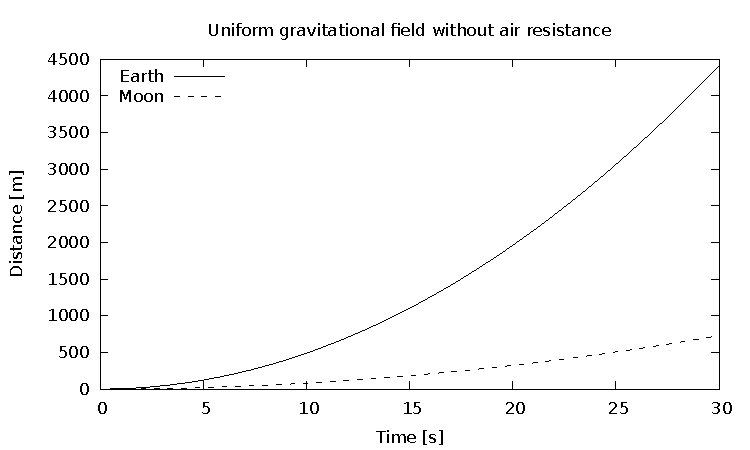
\includegraphics{gnuplot-bw}
% 	\caption{Černobílá varianta obrázku generovaného programem Gnuplot}\label{fig:gnuplot-bw}
% \end{figure}
% 
% \begin{figure}\centering
% 	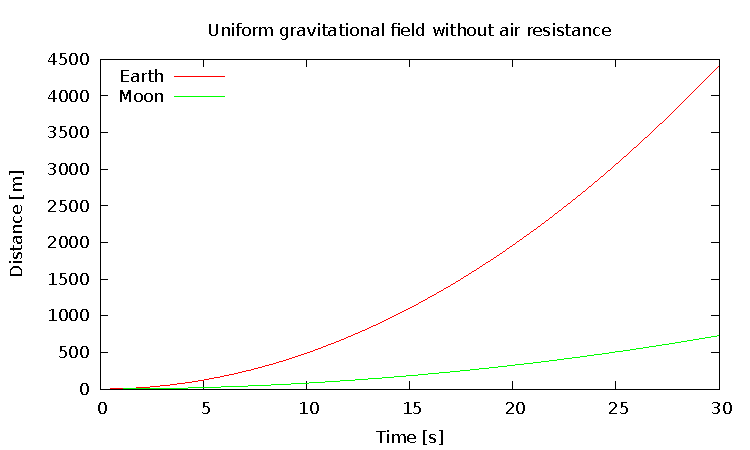
\includegraphics{gnuplot-col}
% 	\caption{Barevná varianta obrázku generovaného programem Gnuplot}\label{fig:gnuplot-col}
% \end{figure}
% 
% 
% \subsection{Tabulky}
% 
% Tabulky lze zadávat různě, např. v~prostředí \verb|tabular|, avšak pro jejich vkládání platí to samé, co pro obrázky -- použijte plovoucí prostředí, v~tomto případě \verb|table|. Například tabulka \ref{tab:matematika} byla vložena tímto způsobem.
% 
% \begin{table}\centering
% 	\caption[Příklad tabulky]{Zadávání matematiky}\label{tab:matematika}
% 	\begin{tabular}{|l|l|c|c|}\hline
% 		Typ		& Prostředí		& \LaTeX{}ovská zkratka	& \TeX{}ovská zkratka	\tabularnewline \hline \hline
% 		Text		& \verb|math|		& \verb|\(...\)|	& \verb|$...$|		\tabularnewline \hline
% 		Displayed	& \verb|displaymath|	& \verb|\[...\]|	& \verb|$$...$$|	\tabularnewline \hline
% 	\end{tabular}
% \end{table}able}
% 
% % % % % % % % % % % % % % % % % % % % % % % % % % % % 

\chapter{Obsah přiloženého CD}

%upravte podle skutecnosti

\begin{figure}
	\dirtree{%
		.1 readme.txt\DTcomment{stručný popis obsahu CD}.
		.1 exe\DTcomment{adresář se spustitelnou formou implementace}.
		.1 src.
		.2 impl\DTcomment{zdrojové kódy implementace}.
		.2 thesis\DTcomment{zdrojová forma práce ve formátu \LaTeX{}}.
		.1 text\DTcomment{text práce}.
		.2 thesis.pdf\DTcomment{text práce ve formátu PDF}.
		.2 thesis.ps\DTcomment{text práce ve formátu PS}.
	}
\end{figure}

\end{document}
